\chapter{Aquifer test - Data analysis overview}
\label{chapter:Extense_fieldwork_analysis}

This appendix accommodates an overview in fieldwork data analysis. Section \ref{sec:python_analysis} contains multiple distinctive python script applied in fieldwork data analysis. The results of all determined geohydrological parameter values (25 approaches for each pumping test / location) can be found in Section \ref{sec:data_analysis overview}.   

\section{Example Python scripts}
\label{sec:python_analysis}
\bigskip
\textbf{Example Python script - Theis's method}
\begin{python}[h!]
def drawdown(t, T, S):
    s = Q / (4 * np.pi * T) * exp1(r ** 2 * S / (4 * T *t))
    s[t > toff] -= Q / (4 * np.pi * T) * exp1(r ** 2 * S / (4 * T *(t[t>toff] - toff)))   
    return s
\end{python}

Where $s$ (m) is the drawdown at distance $r$ (m) from the well, $Q$ (m$^{3}$) is the constant well discharge , $KD$ (m$^{2}$/d) is the aquifer transmissivity ($KD$ = $T$), $S$ (-) is the aquifer storativity, $t$ (d) is the time measured from the start of pumping and $exp1$ is the exponential integral. The drawdown measurements in this research are limited to in-well measurements. The distance $r$ in Theis's equation is assumed to be the length of the well radius (0.0635 m). \\

\textbf{Example Python script - \texttt{Fmin-RMSE} optimization} \\
An example Python implementation of \texttt{Fmin} optimization is given below. It shows an optimization of a two layered model, containing five parameters ($T$ and $S$ values for two model layers and well skin resistance). 

\begin{python}[h!]
def optimTTim_Qvar(params, t, meas):
    kaq = np.zeros(2)
    Saq = np.zeros(2)
    kaq[0] = params[0]             
    kaq[1] = params[1]
    Saq[0] = params[2]
    Saq[1] = params[3]
    res = params[4]
    s = drawdownTTim_Qvar(t, kaq, Saq, res)
    error = np.sqrt(np.mean((s-meas)**2)) 
    return error

xopt = fmin(optimTTim_Qvar, x0=[10, 10, .01, .001, 0.1], args=(to[mask], do[mask]), xtol=1e-4)
\end{python}

Where $kaq[0]$ and $kaq[1]$ (m/d) are respectively the hydraulic conductivities of the first and second layer, $Saq[0]$ and $Saq[1]$ (m/d) are the storativities (-) of the first and second layer, $res$ (d) is the well skin resistance, $s$ (m) is the modelled (optimal) drawdown, $error$ (m) is the RMSE objective function and $x0$ contains the ordered initial parameter conditions. \\

\textbf{Example Python script - TTim \texttt{Calibrate} optimization} \\
In the Python script below, an example of the TTim \texttt{Calibrate} function is given. It is the same example as mentioned in the \texttt{Fmin} optimization above. 

\begin{python}[h!]
cal = Calibrate(mlc)
cal.parameter(name='kaq0', layer=0, initial=10, pmin=0)
cal.parameter(name='kaq1', layer=1, initial=10, pmin=0)
cal.parameter(name='Saq0', layer=0, initial=.01, pmin=0, pmax=0.3)
cal.parameter(name='Saq1', layer=1, initial=.001, pmin=0, pmax=0.3)
cal.parameter(name='res', par=wc.res, initial=0.1)
cal.series(name='obs3', x=ro, y=0, layer=[0,1], t=to[mask], h=-do[mask])
cal.fit()
\end{python}

Where $'kaq0'$ and $'kaq1'$ (m/d) are respectively the hydraulic conductivities of the first and second layer, $'Saq0'$ and $'Saq1'$ (m/d) are the storativities (-) of the first and second layer, $'res'$ (d), $x$ (or $y$) (m) is the radius of the well, $layer$ contains the layer numbers of the 'active' connected layer, $iniitial$ is the initial parameter condition and $pmin$ and $pmax$ are the predefined 'allowed' minimum and maximum  values for that particular parameter.

\section{Data analysis overview}
\label{sec:data_analysis overview}
Each dataset (location specific) is analysed by multiple distinctive simulations. The simulations are distinctive in: theoretical model ( single layer, double layer and double layer and partial penetration of the well), method (analytical Theis's method (single layer only), TTim) and optimization function (\texttt{Fmin-RMSE} and TTim \texttt{Calibrate})). In the TTim analysis an additional distinction is made between analysis by the use of (a) actual borehole storage and no well resistance, (b) optimal borehole storage and no well resistance, (c) actual borehole storage and optimal well resistance, (d) optimal borehole storage and optimal well resistance. Summarized, the location specific datasets are subjected to 25 different approaches in analysis; analytical (1x), Fmin-RMSE (4x3 = 12x) and TTim Calibrate (4x3 = 12x). Table \ref{tab:overview_table} contains an overview of the approaches in fieldwork data analysis.   

\begin{table}[h!]
\small
\centering
\caption{Overview - approaches in fieldwork data analysis}
\label{tab:overview_table}
\begin{tabular}{l|c|c|c|c}
\hline 
\textbf{}                 & \textbf{}        & \textbf{Actual bor stor} & \textbf{Opt bor stor} & \textbf{Opt well res}   \\ \hline \hline
Analytical                &                  & -                        & -                     & -          \\ \hline
Fmin-RMSE                 & a                & x                        & -                     & -          \\
                          & b                & -                        & x                     & -          \\
                          & c                & x                        & -                     & x          \\
                          & d                & -                        & x                     & x          \\ \hline
TTim Cal                  & a                & x                        & -                     & -          \\
                          & b                & -                        & x                     & -          \\
                          & c                & x                        & -                     & x          \\
                          & d                & -                        & x                     & x          \\ \hline    
\end{tabular}
\end{table}
* where the different approaches of the \texttt{Fmin-RMSE} and TTim \texttt{Calibrate} (a-d) are analysed in combination with a single layer system, a double layer system and a system with a two layers and partial penetration of the well. \\

The results of all determined geohydrological parameter values can (by location) be found below. 

\clearpage\subsection{Location: Bingo}
\label{subsec:Bingo_overview}

\begin{figure}[h!]
	\centering
	\begin{subfigure}[b]{0.65\linewidth}
		\centering\includegraphics[width=\linewidth]{Bingo_1lay_fmin}
		\captionsetup{justification=centering}		
		\caption{\label{fig:Bingo_1lay_fmin}}
		\end{subfigure}\vfill
	\begin{subfigure}[b]{0.65\linewidth}
		\centering\includegraphics[width=\linewidth]{Bingo_1lay_cal}
		\captionsetup{justification=centering}		
		\caption{\label{fig:Bingo_1lay_cal}}
		\end{subfigure}
	\captionsetup{justification=centering}	
	\caption{Bingo single layer fieldwork data analysis by the optimization (\subref{fig:Bingo_1lay_fmin}) fmin-RMSE method and (\subref{fig:Bingo_1lay_cal}) TTim calibration method} 
	\label{fig:Bingo_1lay_analysis}
\end{figure} 

\begin{figure}[h!]
	\centering
	\begin{subfigure}[b]{0.65\linewidth}
		\centering\includegraphics[width=\linewidth]{Bingo_2lay_fmin}
		\captionsetup{justification=centering}		
		\caption{\label{fig:Bingo_2lay_fmin}}
		\end{subfigure}\vfill
	\begin{subfigure}[b]{0.65\linewidth}
		\centering\includegraphics[width=\linewidth]{Bingo_2lay_cal}
		\captionsetup{justification=centering}		
		\caption{\label{fig:Bingo_2lay_cal}}
		\end{subfigure}
	\captionsetup{justification=centering}	
	\caption{Bingo double layer fieldwork data analysis by the optimization (\subref{fig:Bingo_2lay_fmin}) fmin-RMSE method and (\subref{fig:Bingo_2lay_cal}) TTim calibration method} 
	\label{fig:Bingo_2lay_analysis}
\end{figure} 

\begin{figure}[h!]
	\centering
	\begin{subfigure}[b]{0.65\linewidth}
		\centering\includegraphics[width=\linewidth]{Bingo_3lay_fmin}
		\captionsetup{justification=centering}		
		\caption{\label{fig:Bingo_3lay_fmin}}
		\end{subfigure}\vfill
	\begin{subfigure}[b]{0.65\linewidth}
		\centering\includegraphics[width=\linewidth]{Bingo_3lay_cal}
		\captionsetup{justification=centering}		
		\caption{\label{fig:Bingo_3lay_cal}}
		\end{subfigure}
	\captionsetup{justification=centering}	
	\caption{Bingo partially penetrating double layer fieldwork data analysis by the optimization (\subref{fig:Bingo_3lay_fmin}) fmin-RMSE method and (\subref{fig:Bingo_3lay_cal}) TTim calibration method} 
	\label{fig:Bingo_3lay_analysis}
\end{figure} 

\clearpage

\begin{figure}[h!]
	\centering
	\begin{subfigure}[b]{\linewidth}
		\centering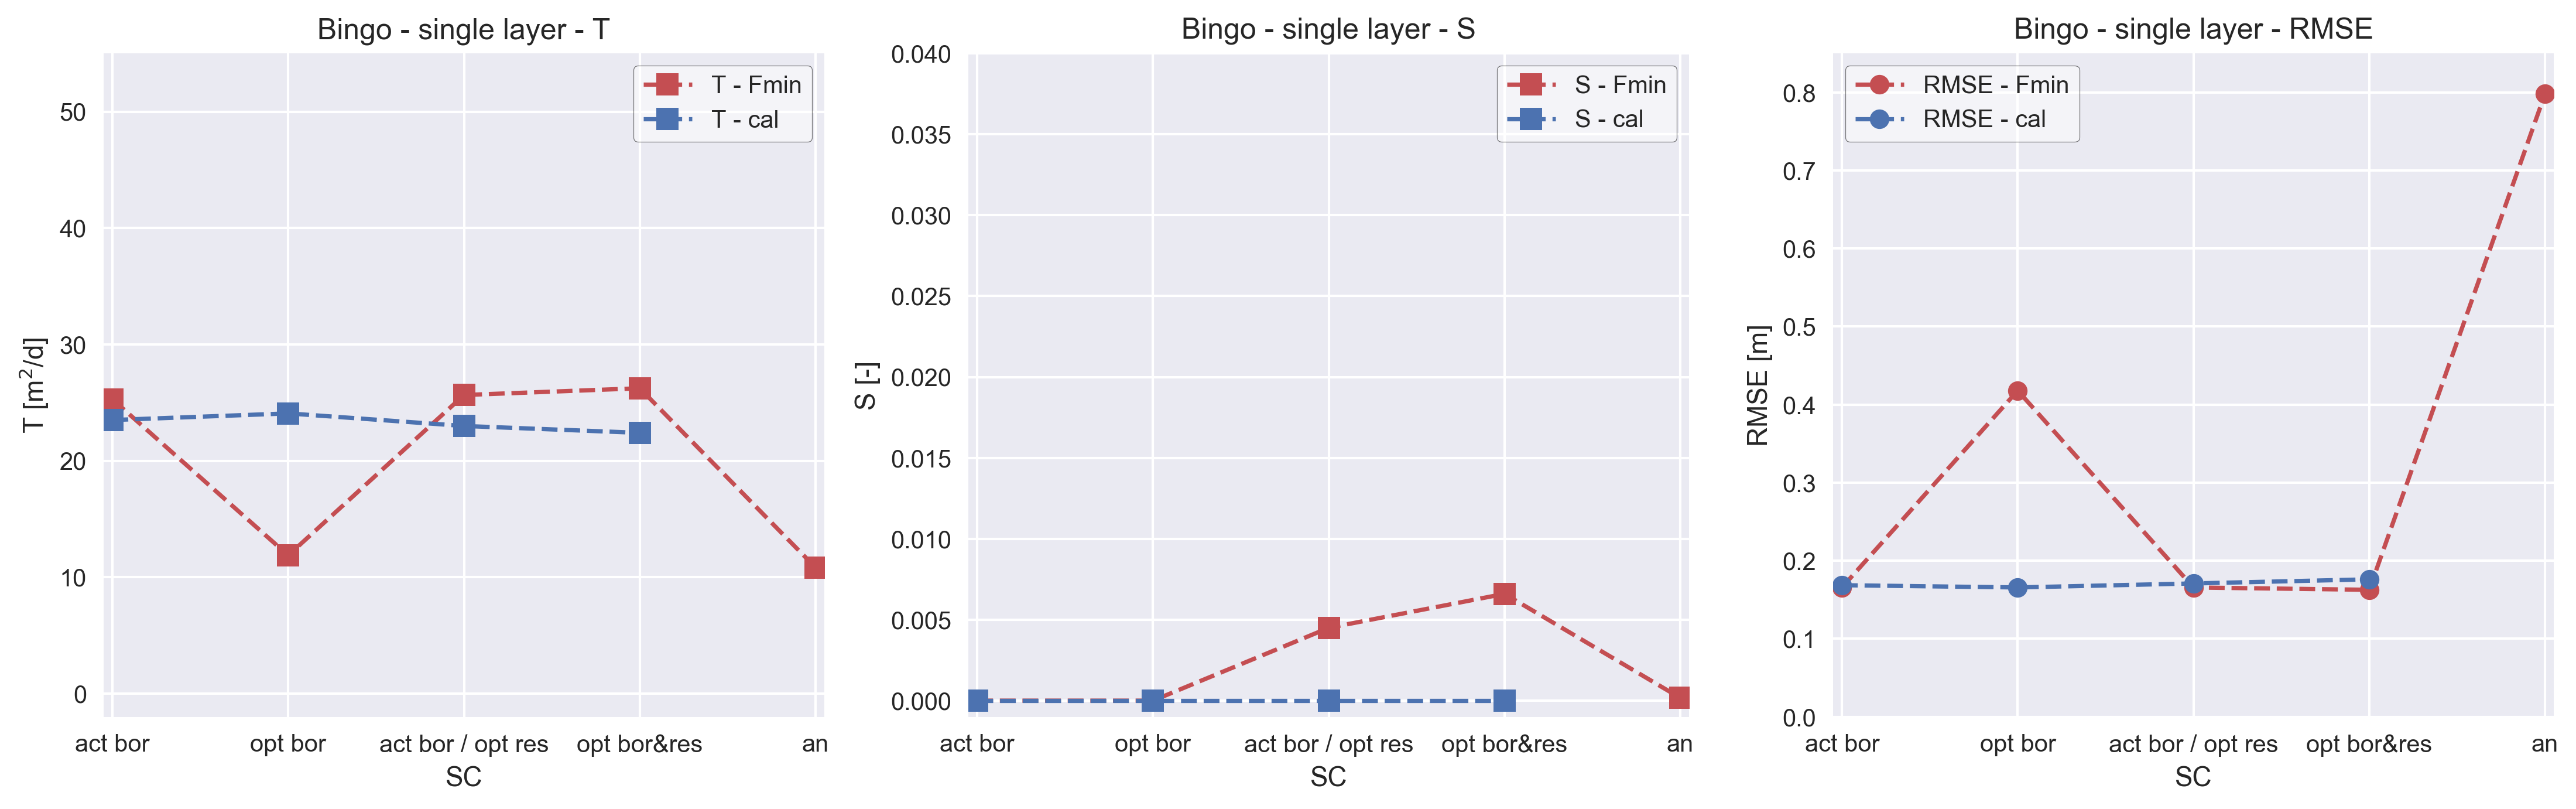
\includegraphics[width=\linewidth]{Bingo_para_results_1lay}
		\captionsetup{justification=centering}		
		\caption{\label{fig:Bingo_para_results_1lay}}
		\end{subfigure}\vfill
	\begin{subfigure}[b]{\linewidth}
		\centering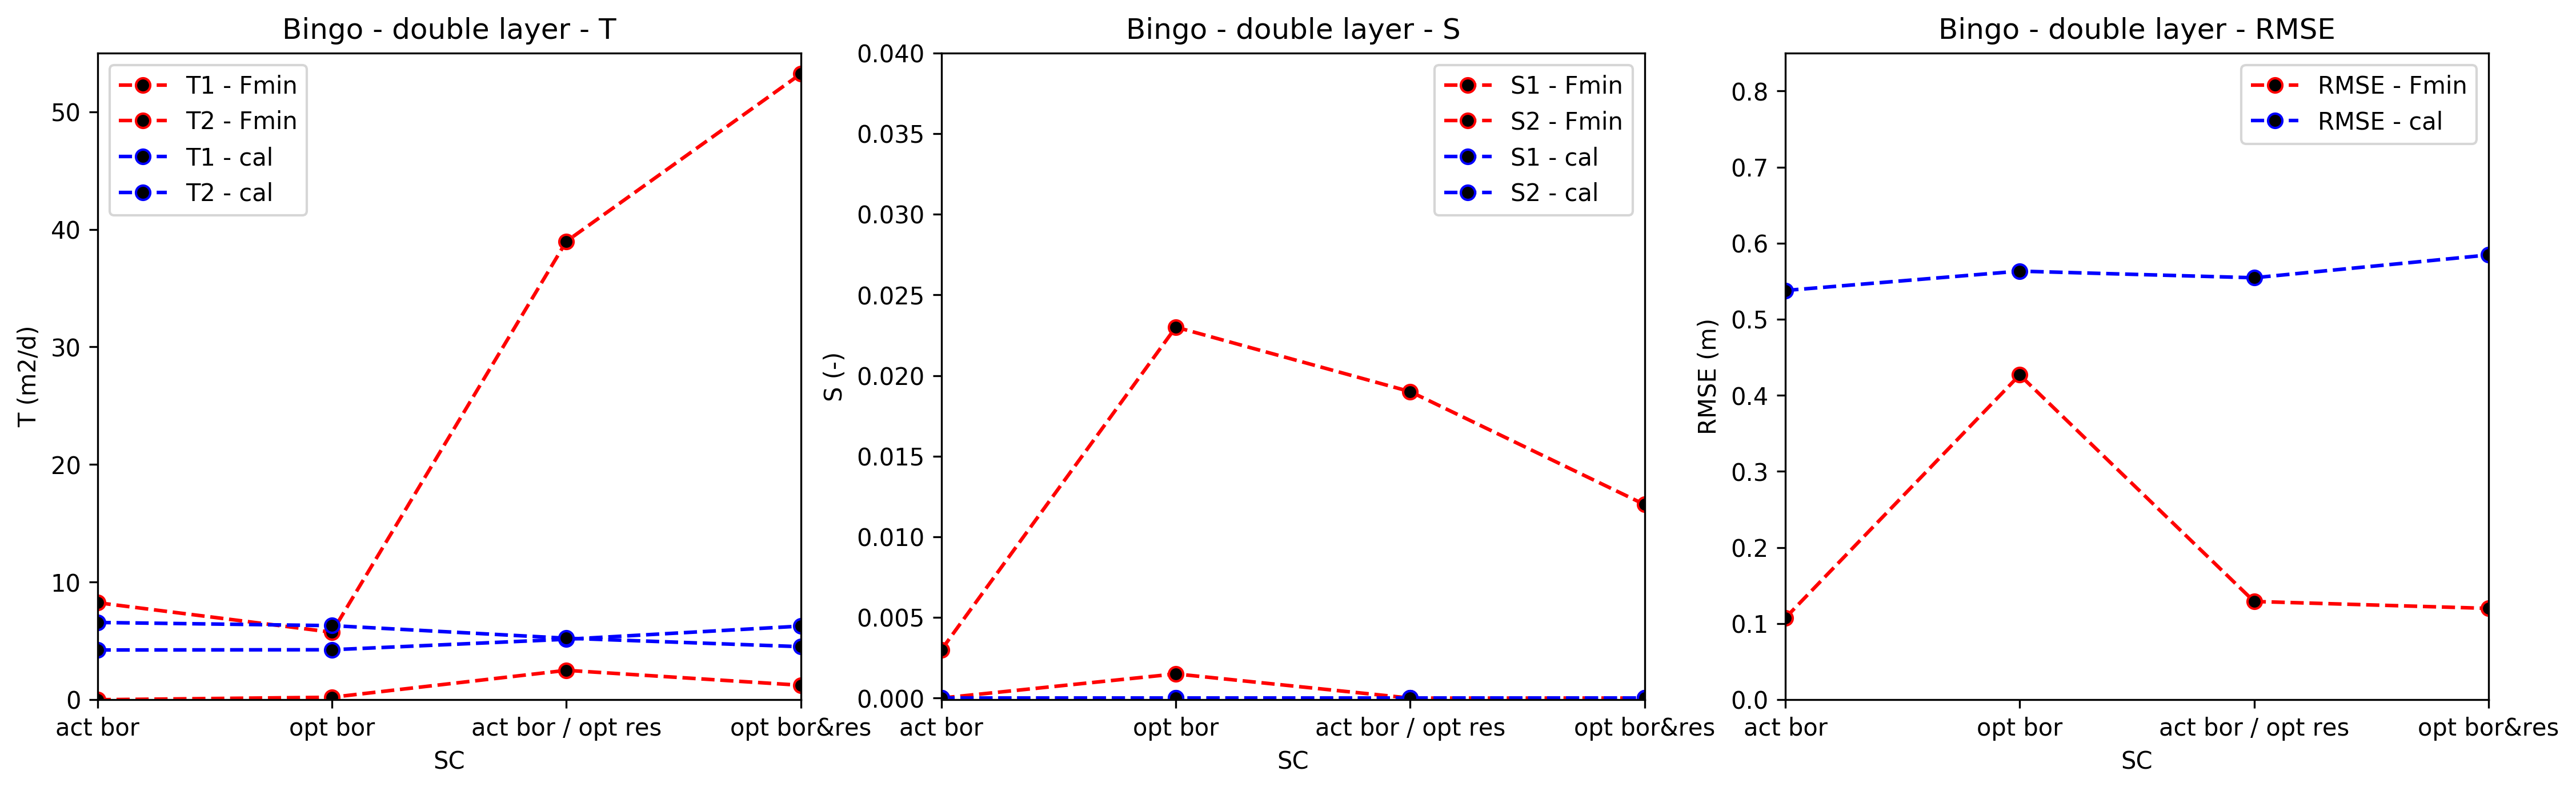
\includegraphics[width=\linewidth]{Bingo_para_results_2lay}
		\captionsetup{justification=centering}		
		\caption{\label{fig:Bingo_para_results_2lay}}
		\end{subfigure}
	\begin{subfigure}[b]{\linewidth}
		\centering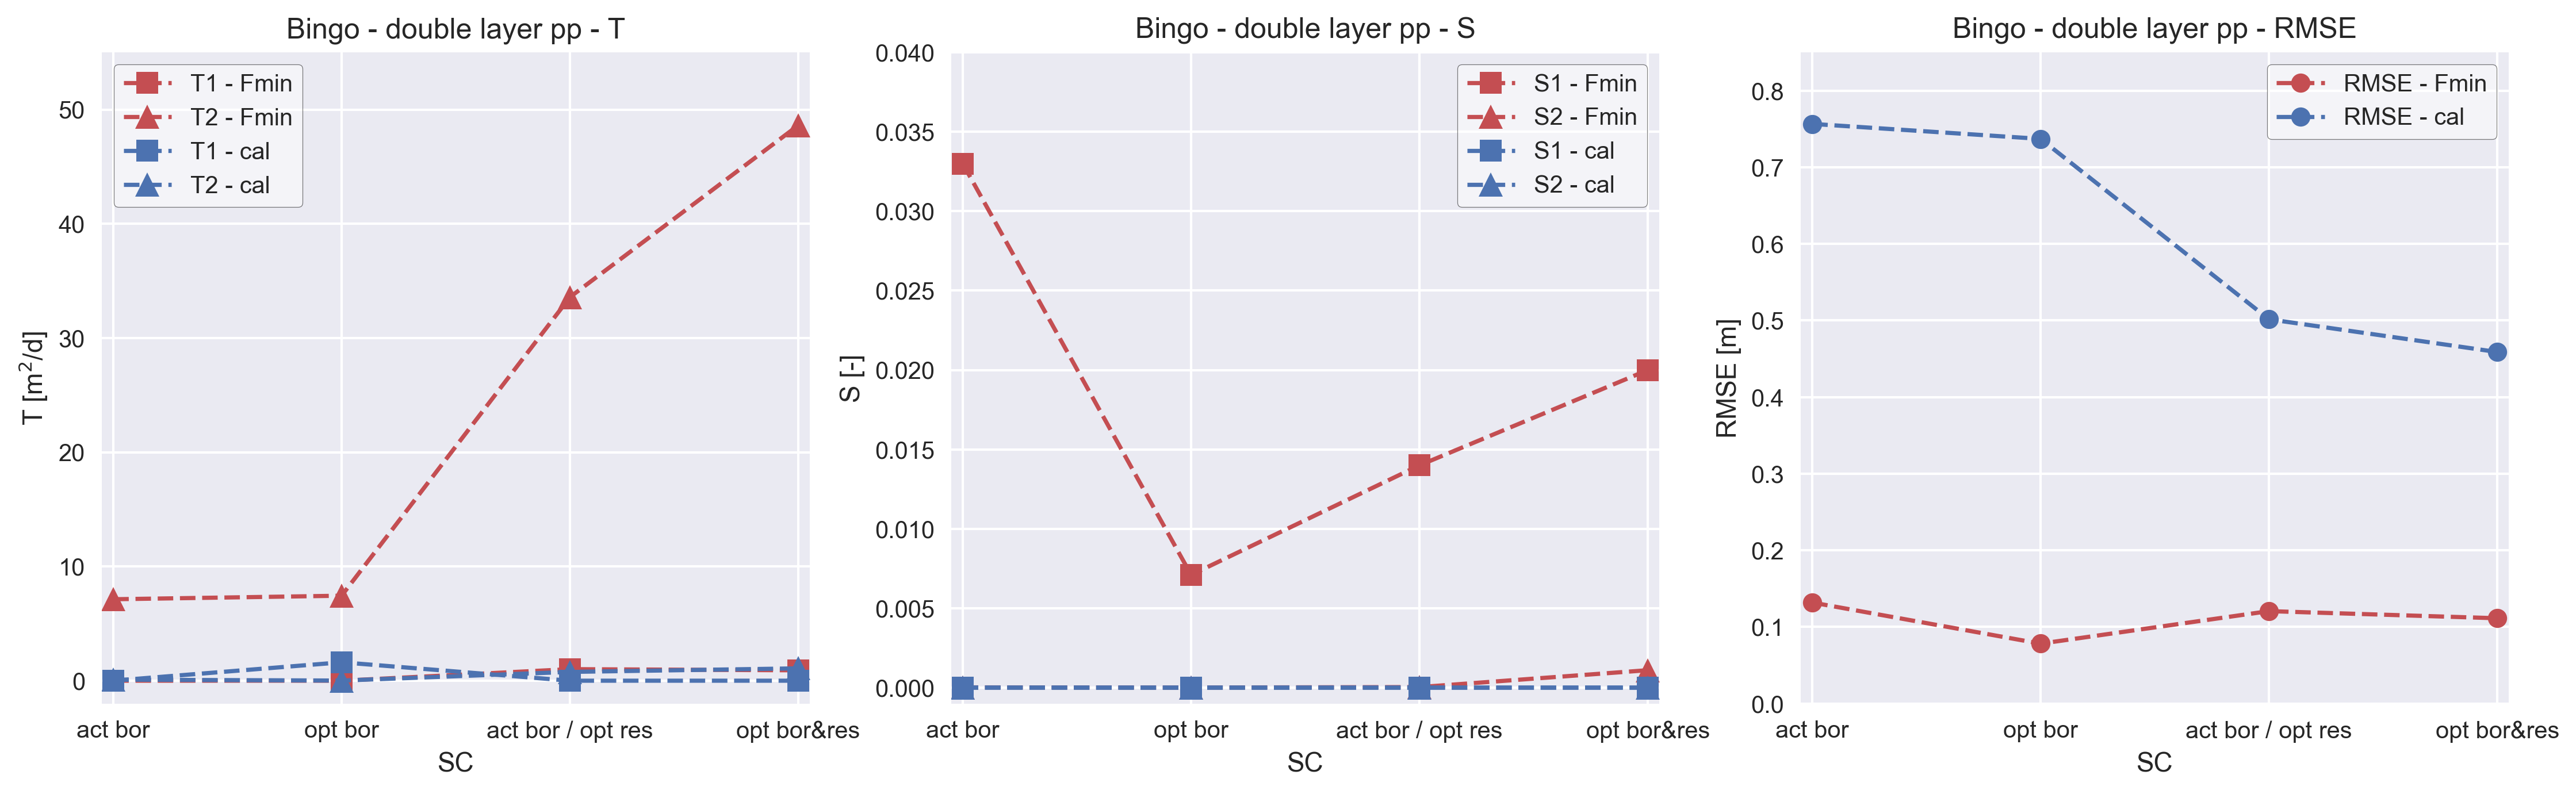
\includegraphics[width=\linewidth]{Bingo_para_results_3lay}
		\captionsetup{justification=centering}		
		\caption{\label{fig:Bingo_para_results_3lay}}
		\end{subfigure}		
	\captionsetup{justification=centering}	
	\caption{Bingo - overview determined (Fmin and Cal) optimal parameter values of (\subref{fig:Bingo_para_results_1lay}) a single layer system, (\subref{fig:Bingo_para_results_2lay}) a double layer system, and (\subref{fig:Bingo_para_results_3lay}) a system with two layers and partial penetration of the well} 
	\label{fig:Bingo_para_results}
\end{figure} 


\clearpage\subsection{Location: Nungo}
\label{subsec:Nungo_overview}
\ bigskip 
Gained fieldwork data at the location Nungo not sufficient for the analysis of geohydrological parameter values.  

\clearpage\subsection{Location: Nyong Nayili}
\label{subsec:Nyong_Nayili_overview}

\begin{figure}[h!]
	\centering
	\begin{subfigure}[b]{0.65\linewidth}
		\centering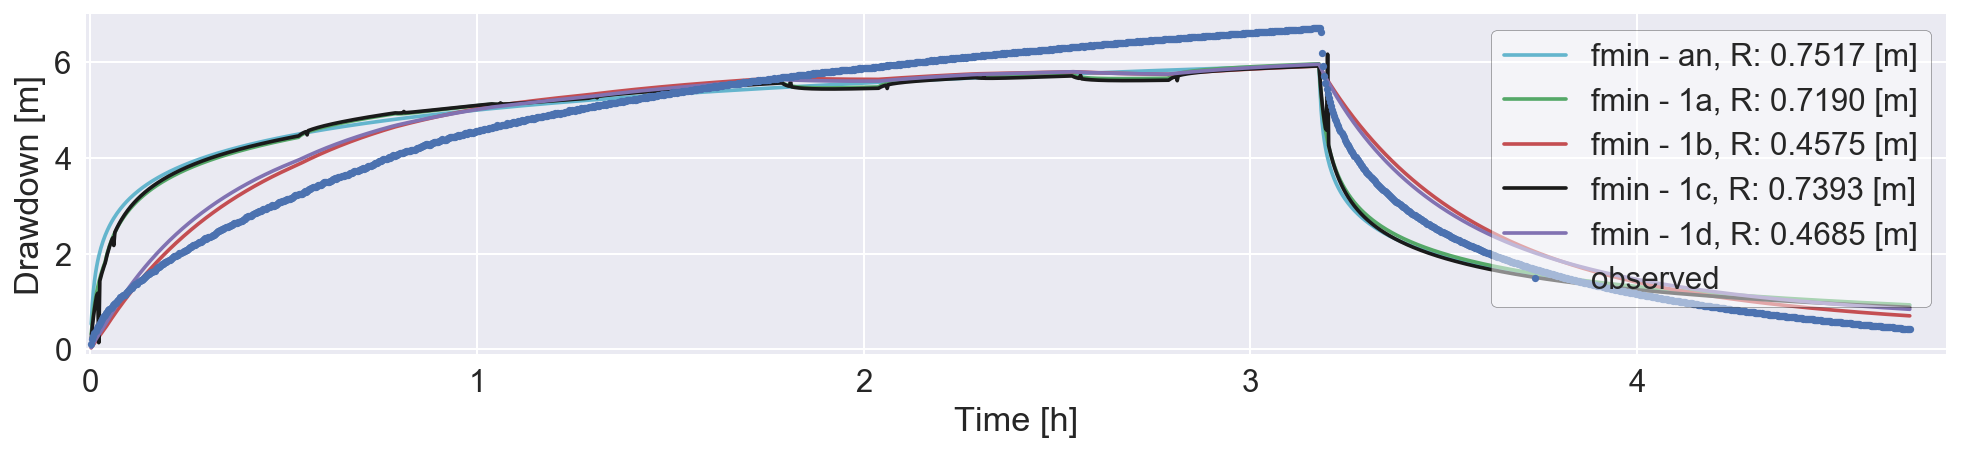
\includegraphics[width=\linewidth]{Nyong_Nayili_1lay_fmin}
		\captionsetup{justification=centering}		
		\caption{\label{fig:Nyong_Nayili_1lay_fmin}}
		\end{subfigure}\vfill
	\begin{subfigure}[b]{0.65\linewidth}
		\centering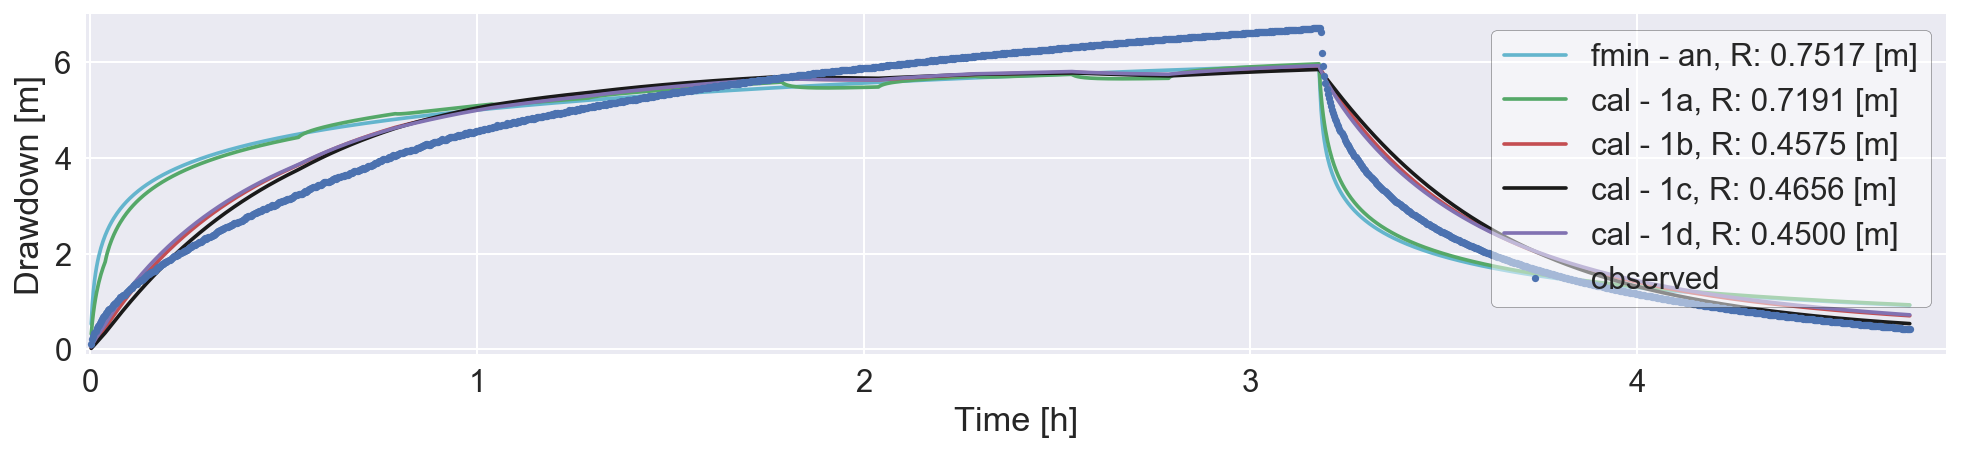
\includegraphics[width=\linewidth]{Nyong_Nayili_1lay_cal}
		\captionsetup{justification=centering}		
		\caption{\label{fig:Nyong_Nayili_1lay_cal}}
		\end{subfigure}
	\captionsetup{justification=centering}	
	\caption{Nyong Nayili single layer fieldwork data analysis by the optimization (\subref{fig:Nyong_Nayili_1lay_fmin}) fmin-RMSE method and (\subref{fig:Nyong_Nayili_1lay_cal}) TTim calibration method} 
	\label{fig:Nyong_Nayili_1lay_analysis}
\end{figure} 

\begin{figure}[h!]
	\centering
	\begin{subfigure}[b]{0.65\linewidth}
		\centering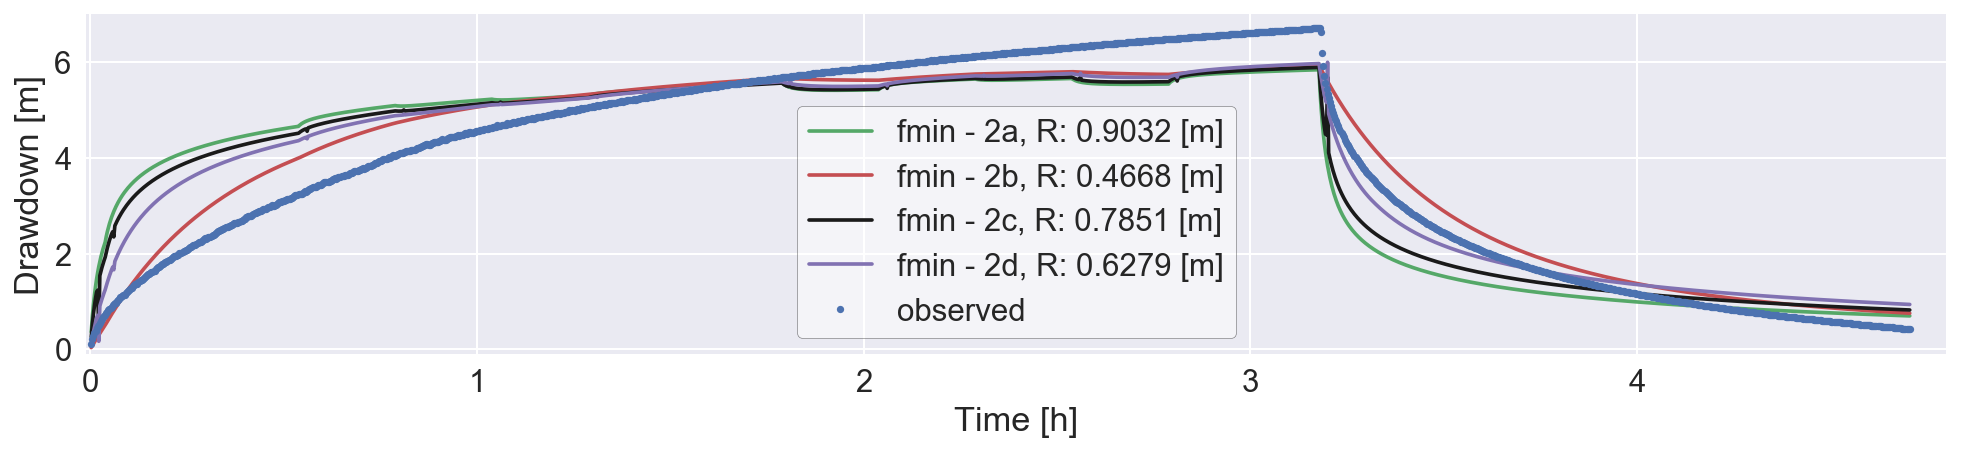
\includegraphics[width=\linewidth]{Nyong_Nayili_2lay_fmin}
		\captionsetup{justification=centering}		
		\caption{\label{fig:Nyong_Nayili_2lay_fmin}}
		\end{subfigure}\vfill
	\begin{subfigure}[b]{0.65\linewidth}
		\centering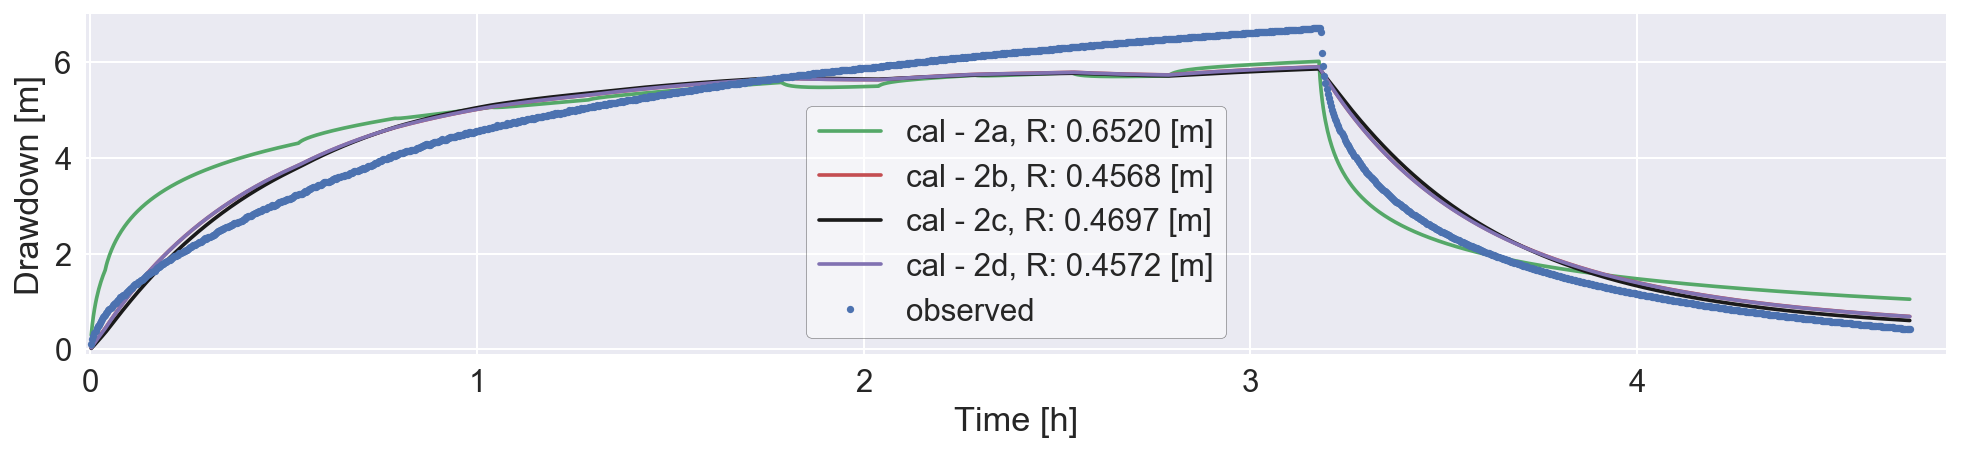
\includegraphics[width=\linewidth]{Nyong_Nayili_2lay_cal}
		\captionsetup{justification=centering}		
		\caption{\label{fig:Nyong_Nayili_2lay_cal}}
		\end{subfigure}
	\captionsetup{justification=centering}	
	\caption{Nyong Nayili double layer fieldwork data analysis by the optimization (\subref{fig:Nyong_Nayili_2lay_fmin}) fmin-RMSE method and (\subref{fig:Nyong_Nayili_2lay_cal}) TTim calibration method} 
	\label{fig:Nyong_Nayili_2lay_analysis}
\end{figure} 

\begin{figure}[h!]
	\centering
	\begin{subfigure}[b]{0.65\linewidth}
		\centering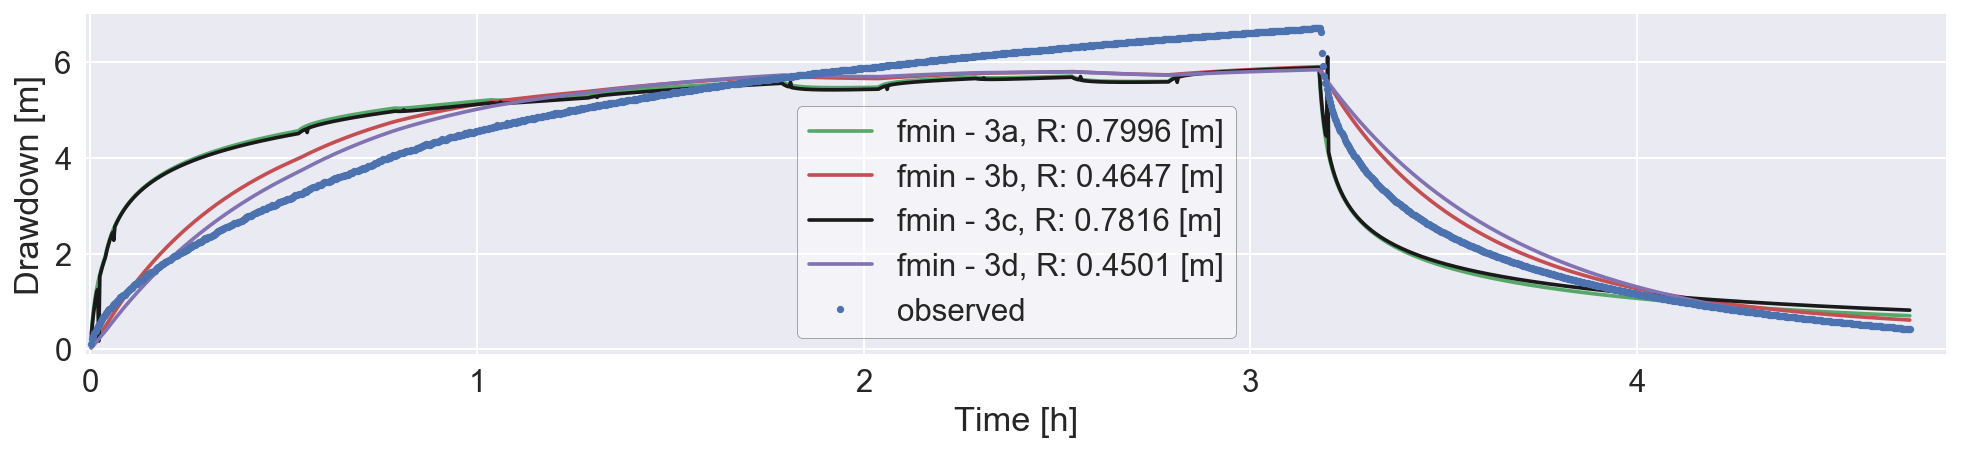
\includegraphics[width=\linewidth]{Nyong_Nayili_3lay_fmin}
		\captionsetup{justification=centering}		
		\caption{\label{fig:Nyong_Nayili_3lay_fmin}}
		\end{subfigure}\vfill
	\begin{subfigure}[b]{0.65\linewidth}
		\centering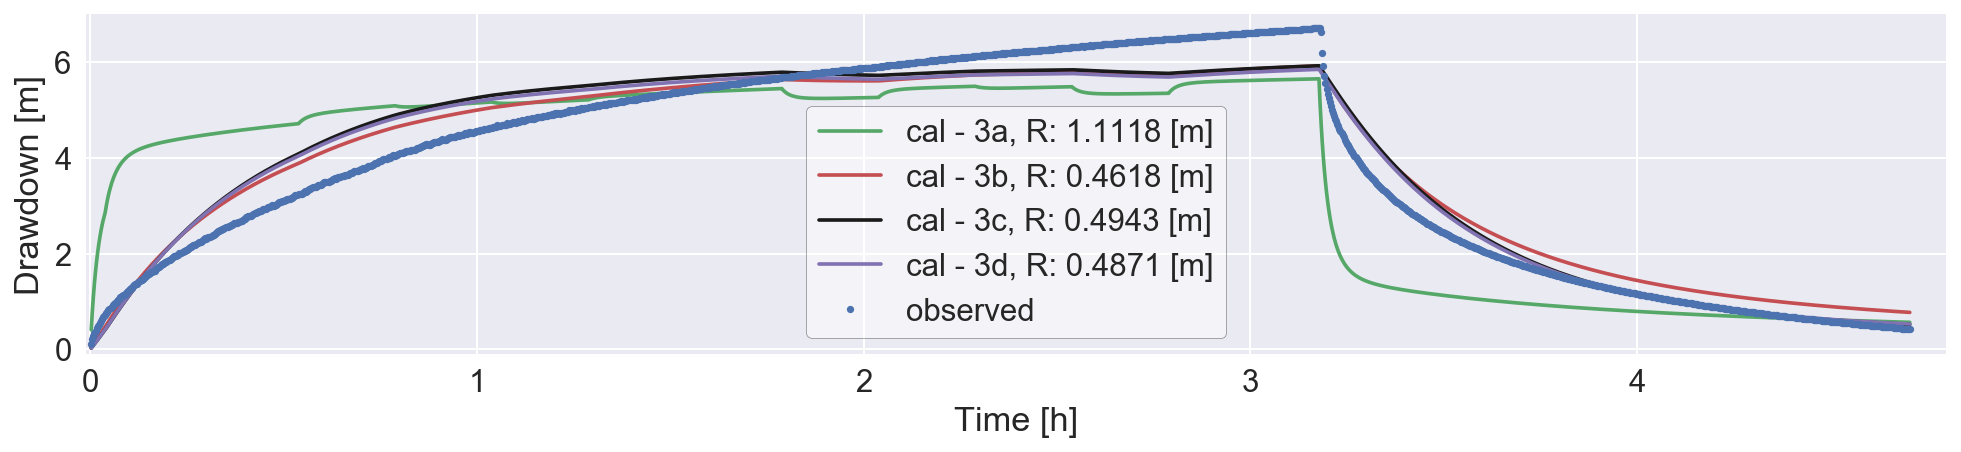
\includegraphics[width=\linewidth]{Nyong_Nayili_3lay_cal}
		\captionsetup{justification=centering}		
		\caption{\label{fig:Nyong_Nayili_3lay_cal}}
		\end{subfigure}
	\captionsetup{justification=centering}	
	\caption{Nyong Nayili partially penetrating double layer fieldwork data analysis by the optimization (\subref{fig:Nyong_Nayili_3lay_fmin}) fmin-RMSE method and (\subref{fig:Nyong_Nayili_3lay_cal}) TTim calibration method} 
	\label{fig:Nyong_Nayili_3lay_analysis}
\end{figure} 

\clearpage

\begin{figure}[h!]
	\centering
	\begin{subfigure}[b]{\linewidth}
		\centering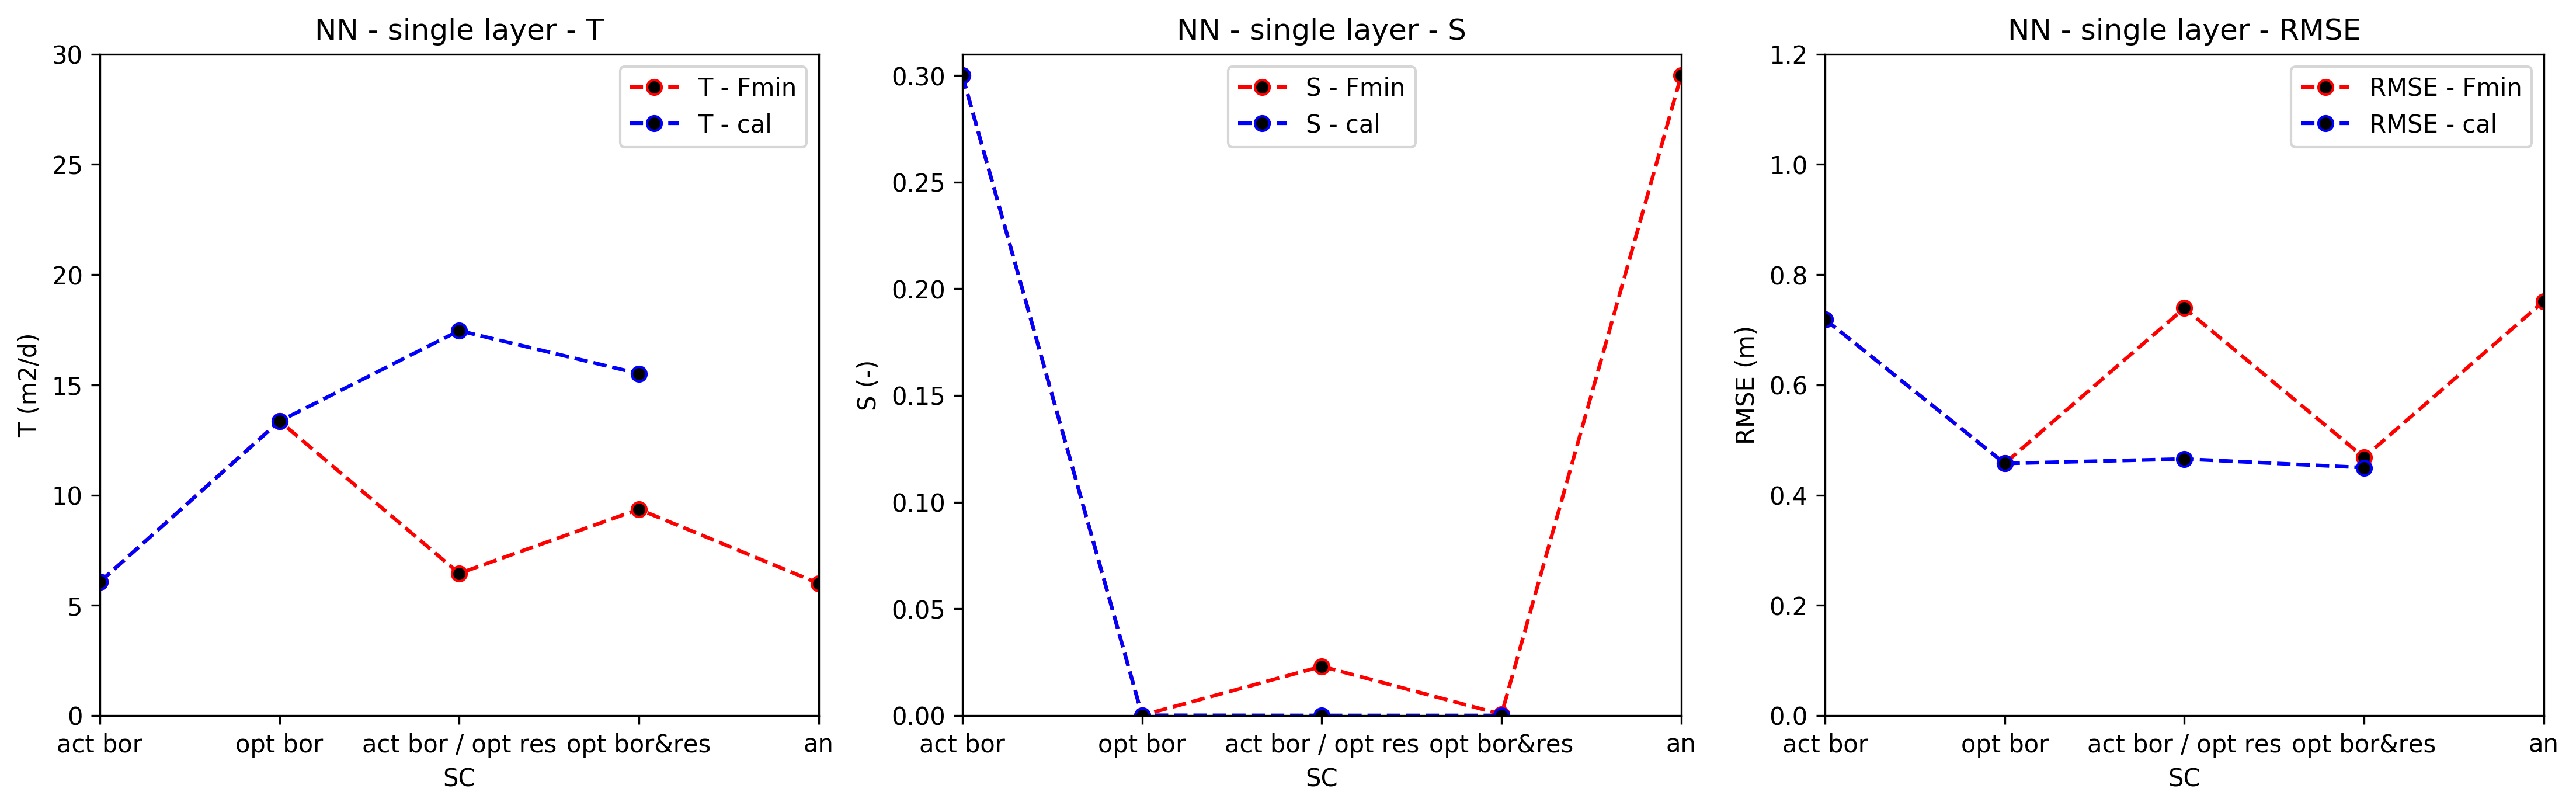
\includegraphics[width=\linewidth]{NN_para_results_1lay}
		\captionsetup{justification=centering}		
		\caption{\label{fig:NN_para_results_1lay}}
		\end{subfigure}\vfill
	\begin{subfigure}[b]{\linewidth}
		\centering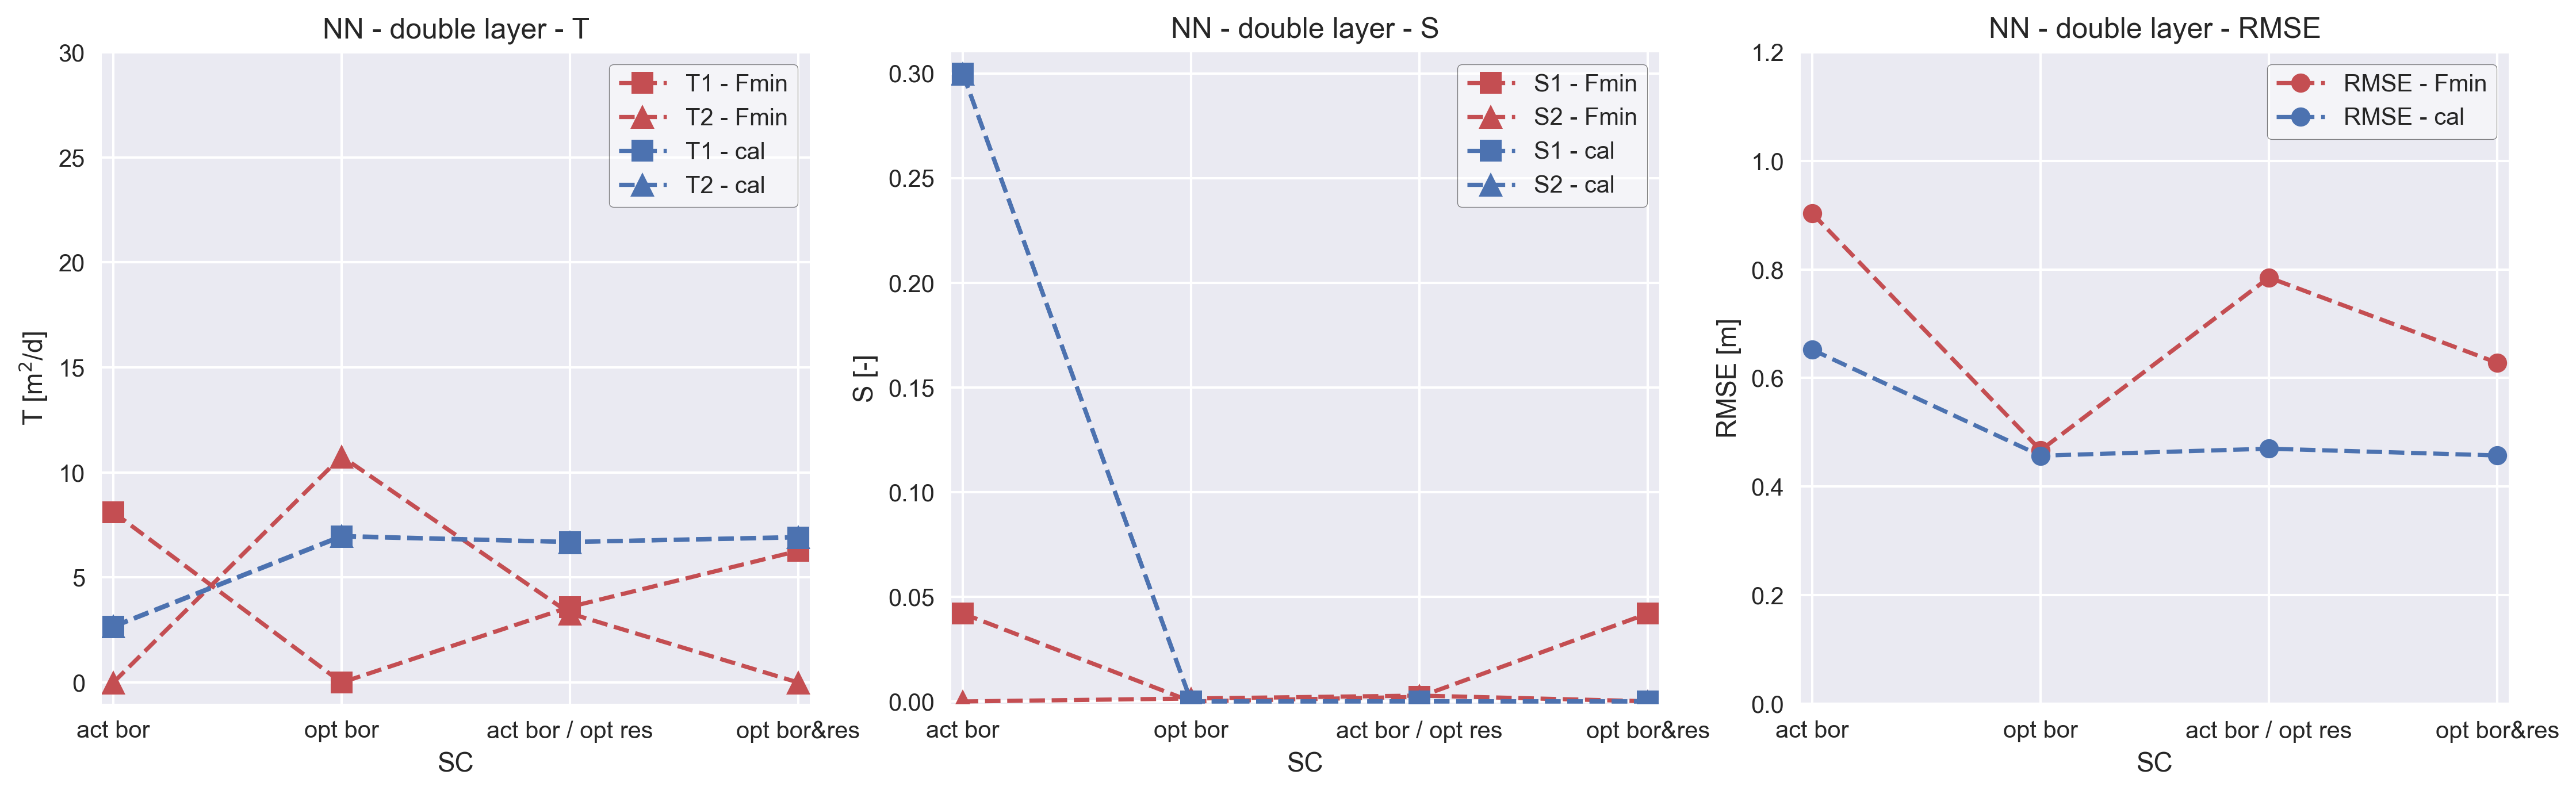
\includegraphics[width=\linewidth]{NN_para_results_2lay}
		\captionsetup{justification=centering}		
		\caption{\label{fig:NN_para_results_2lay}}
		\end{subfigure}
	\begin{subfigure}[b]{\linewidth}
		\centering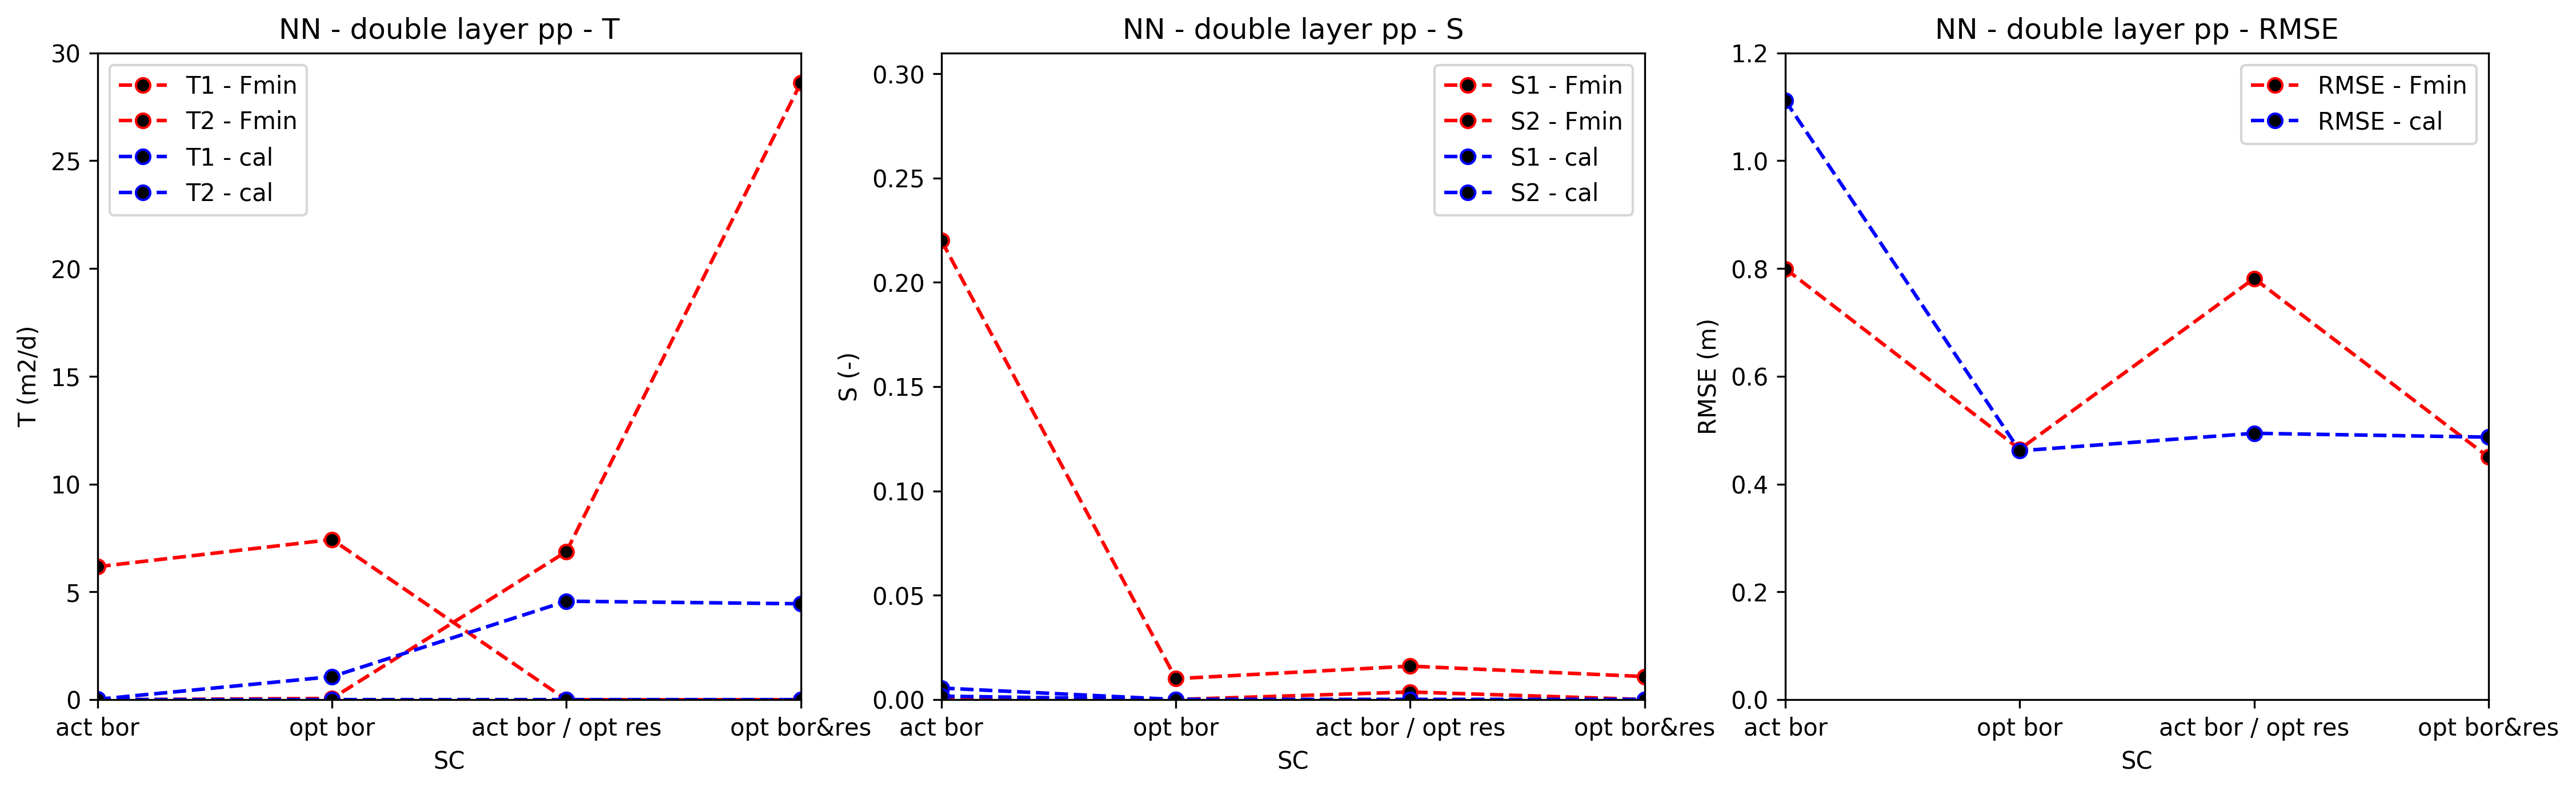
\includegraphics[width=\linewidth]{NN_para_results_3lay}
		\captionsetup{justification=centering}		
		\caption{\label{fig:NN_para_results_3lay}}
		\end{subfigure}		
	\captionsetup{justification=centering}	
	\caption{Nyong Nayili - overview determined (Fmin and Cal) optimal parameter values of (\subref{fig:NN_para_results_1lay}) a single layer system, (\subref{fig:NN_para_results_2lay}) a double layer system, and (\subref{fig:NN_para_results_3lay}) a system with two layers and partial penetration of the well} 
	\label{fig:NN_para_results}
\end{figure} 


\clearpage\subsection{Location: Janga (1/2)}
\label{subsec:Janga1_overview}

\begin{figure}[h!]
	\centering
	\begin{subfigure}[b]{0.65\linewidth}
		\centering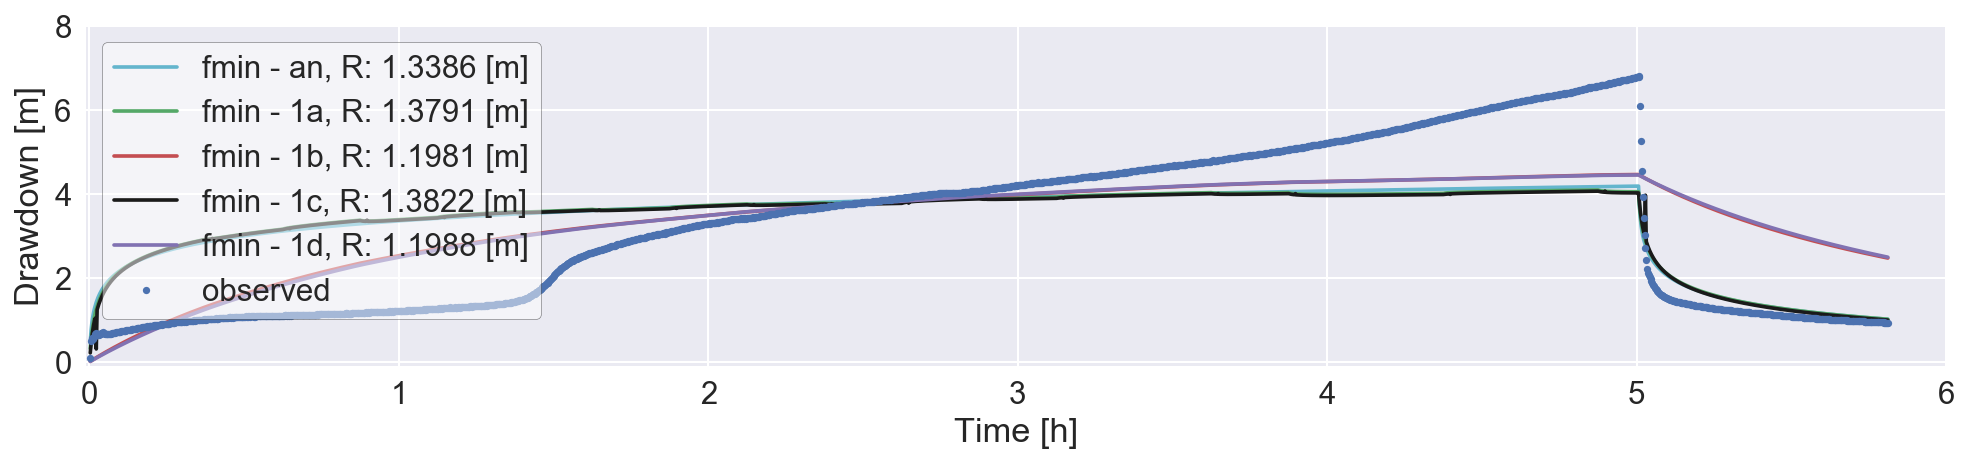
\includegraphics[width=\linewidth]{Janga1_1lay_fmin}
		\captionsetup{justification=centering}		
		\caption{\label{fig:Janga1_1lay_fmin}}
		\end{subfigure}\vfill
	\begin{subfigure}[b]{0.65\linewidth}
		\centering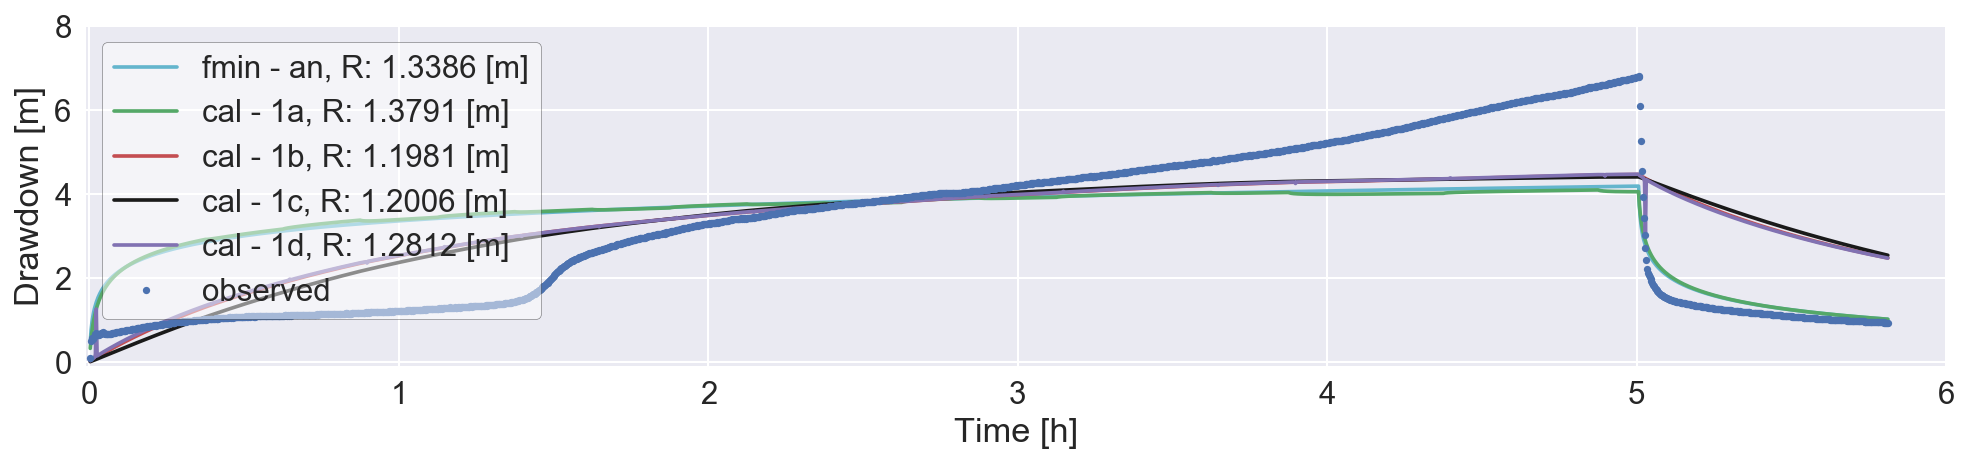
\includegraphics[width=\linewidth]{Janga1_1lay_cal}
		\captionsetup{justification=centering}		
		\caption{\label{fig:Janga1_1lay_cal}}
		\end{subfigure}
	\captionsetup{justification=centering}	
	\caption{Janga first attempt single layer fieldwork data analysis by the optimization (\subref{fig:Janga1_1lay_fmin}) fmin-RMSE method and (\subref{fig:Janga1_1lay_cal}) TTim calibration method} 
	\label{fig:Janga1_1lay_analysis}
\end{figure} 

\begin{figure}[h!]
	\centering
	\begin{subfigure}[b]{0.65\linewidth}
		\centering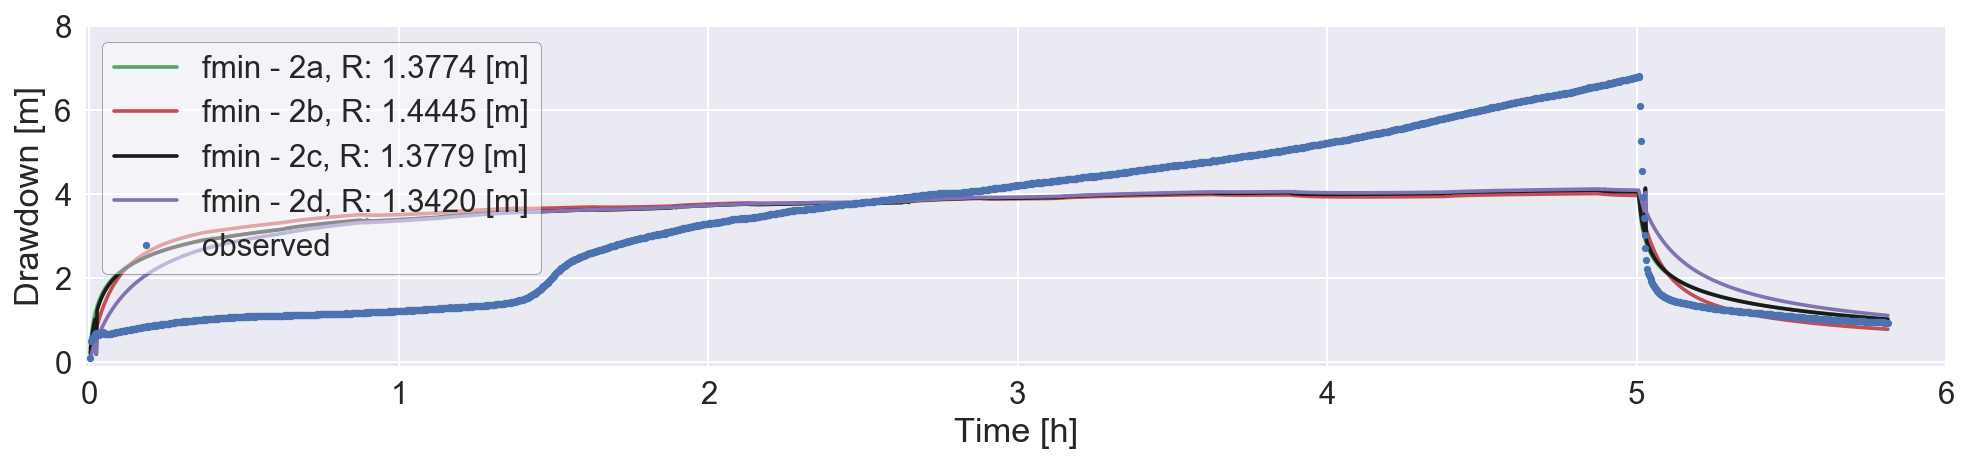
\includegraphics[width=\linewidth]{Janga1_2lay_fmin}
		\captionsetup{justification=centering}		
		\caption{\label{fig:Janga1_2lay_fmin}}
		\end{subfigure}\vfill
	\begin{subfigure}[b]{0.65\linewidth}
		\centering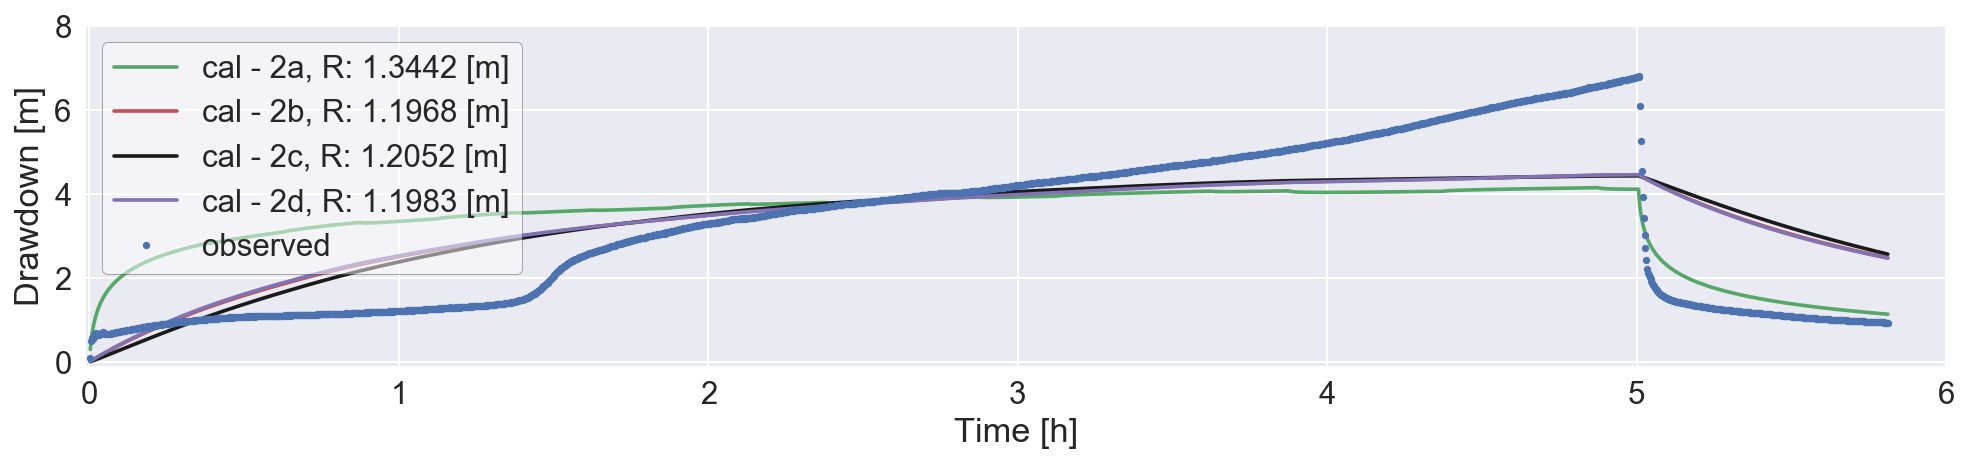
\includegraphics[width=\linewidth]{Janga1_2lay_cal}
		\captionsetup{justification=centering}		
		\caption{\label{fig:Janga1_2lay_cal}}
		\end{subfigure}
	\captionsetup{justification=centering}	
	\caption{Janga first attempt double layer fieldwork data analysis by the optimization (\subref{fig:Janga1_2lay_fmin}) fmin-RMSE method and (\subref{fig:Janga1_2lay_cal}) TTim calibration method} 
	\label{fig:Janga1_2lay_analysis}
\end{figure} 

\begin{figure}[h!]
	\centering
	\begin{subfigure}[b]{0.65\linewidth}
		\centering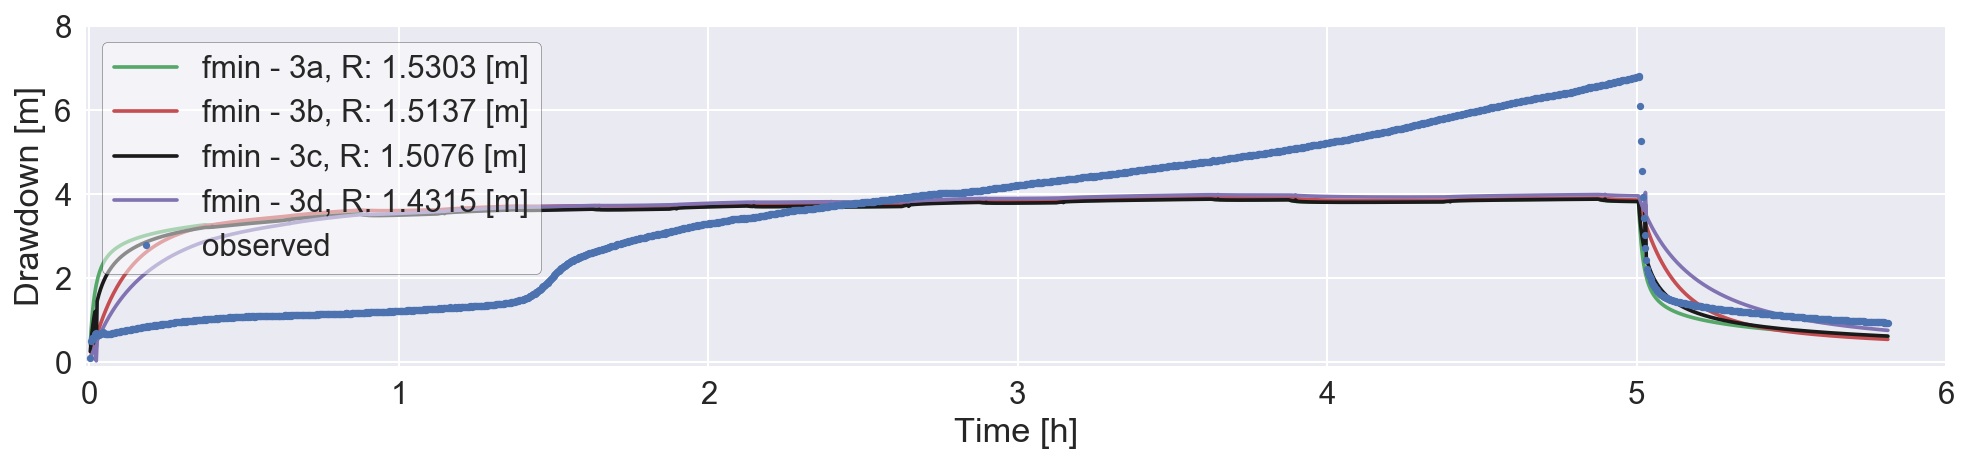
\includegraphics[width=\linewidth]{Janga1_3lay_fmin}
		\captionsetup{justification=centering}		
		\caption{\label{fig:Janga1_3lay_fmin}}
		\end{subfigure}\vfill
	\begin{subfigure}[b]{0.65\linewidth}
		\centering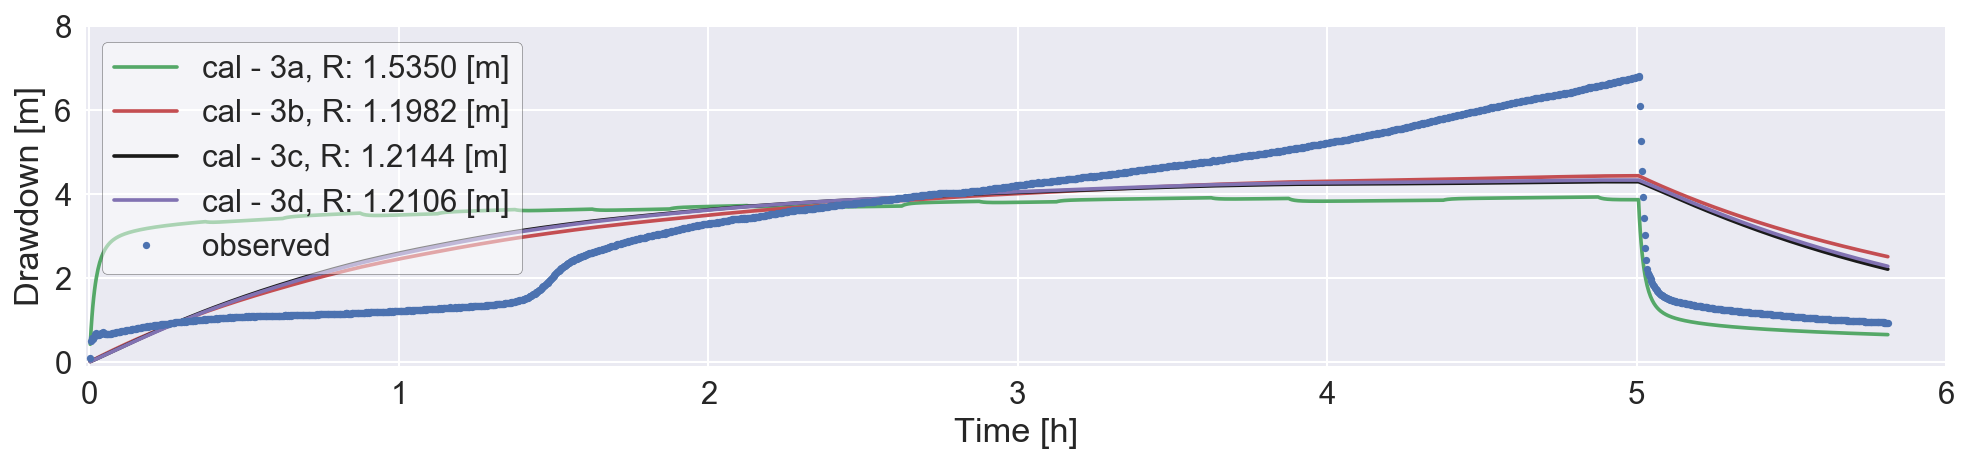
\includegraphics[width=\linewidth]{Janga1_3lay_cal}
		\captionsetup{justification=centering}		
		\caption{\label{fig:Janga1_3lay_cal}}
		\end{subfigure}
	\captionsetup{justification=centering}	
	\caption{Janga first attempt partially penetrating double layer fieldwork data analysis by the optimization (\subref{fig:Janga1_3lay_fmin}) fmin-RMSE method and (\subref{fig:Janga1_3lay_cal}) TTim calibration method} 
	\label{fig:Janga1_3lay_analysis}
\end{figure} 

\clearpage

\begin{figure}[h!]
	\centering
	\begin{subfigure}[b]{\linewidth}
		\centering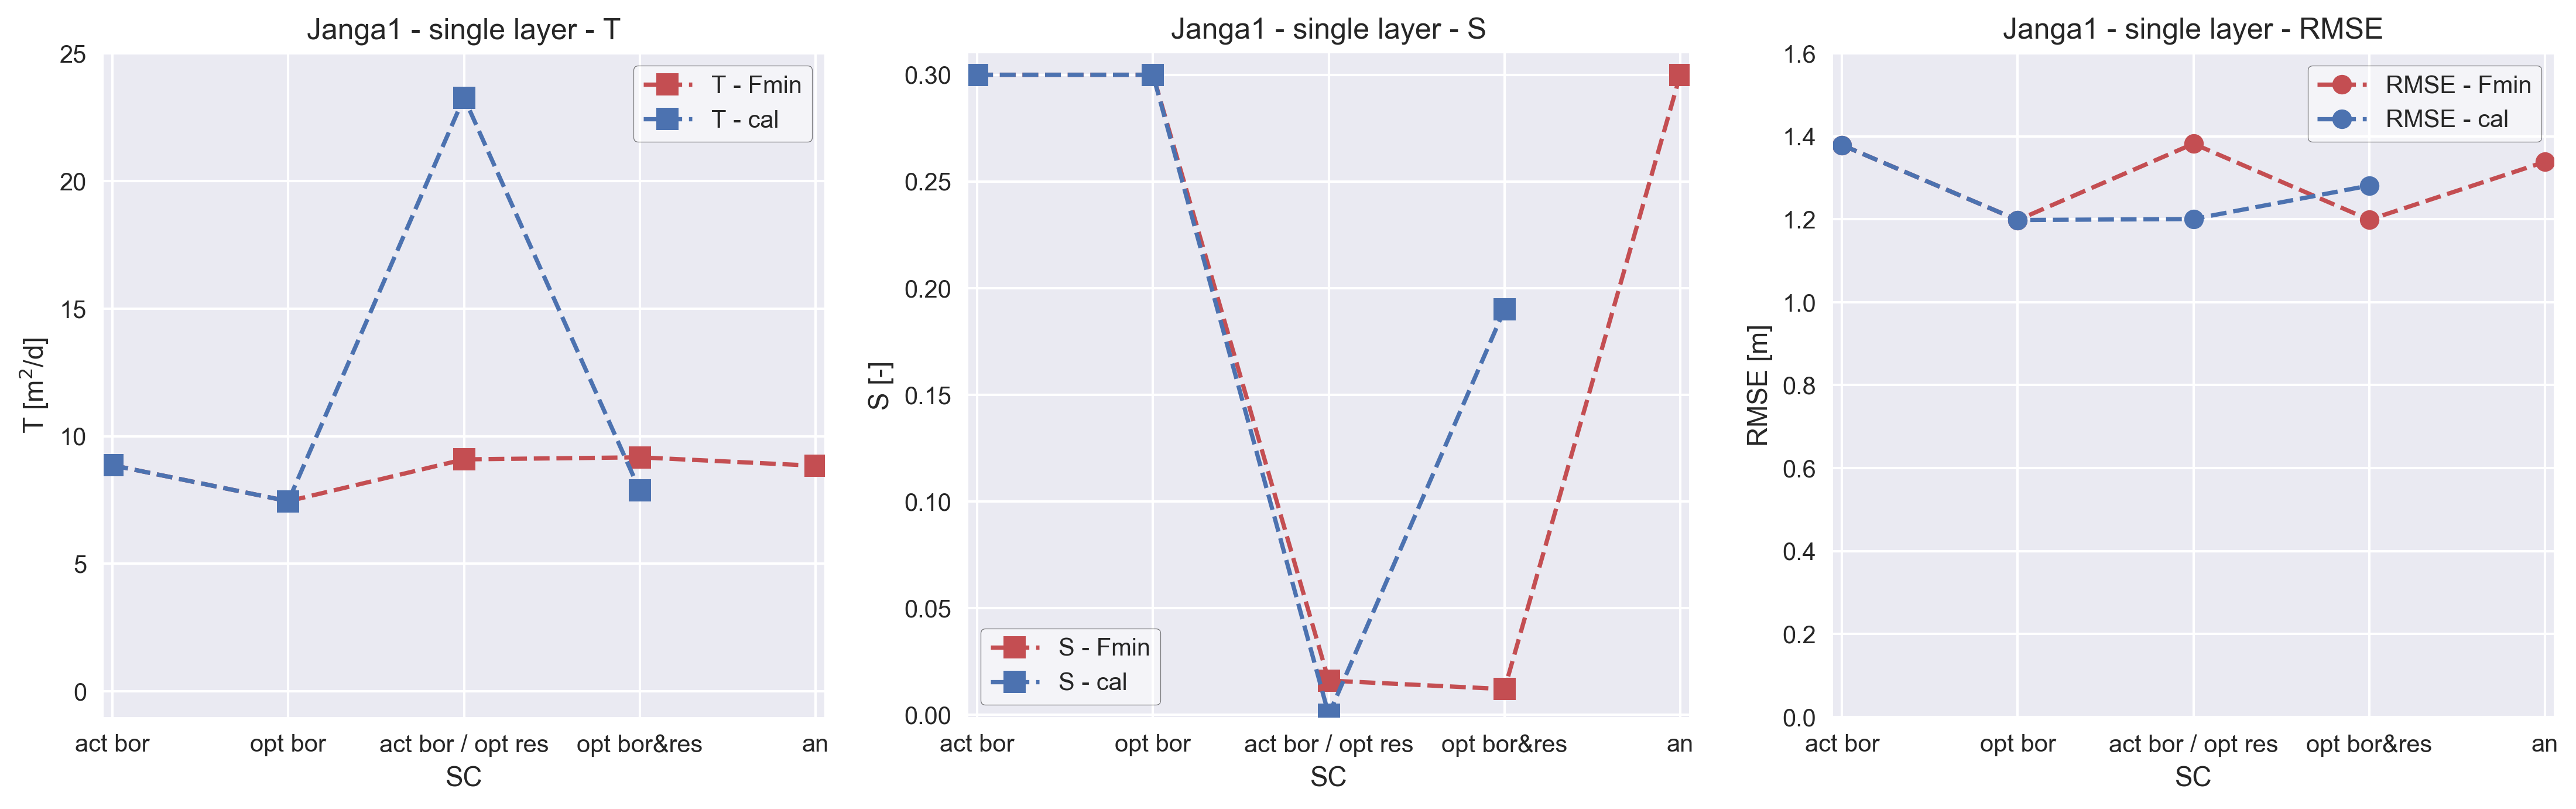
\includegraphics[width=\linewidth]{J1_para_results_1lay}
		\captionsetup{justification=centering}		
		\caption{\label{fig:J1_para_results_1lay}}
		\end{subfigure}\vfill
	\begin{subfigure}[b]{\linewidth}
		\centering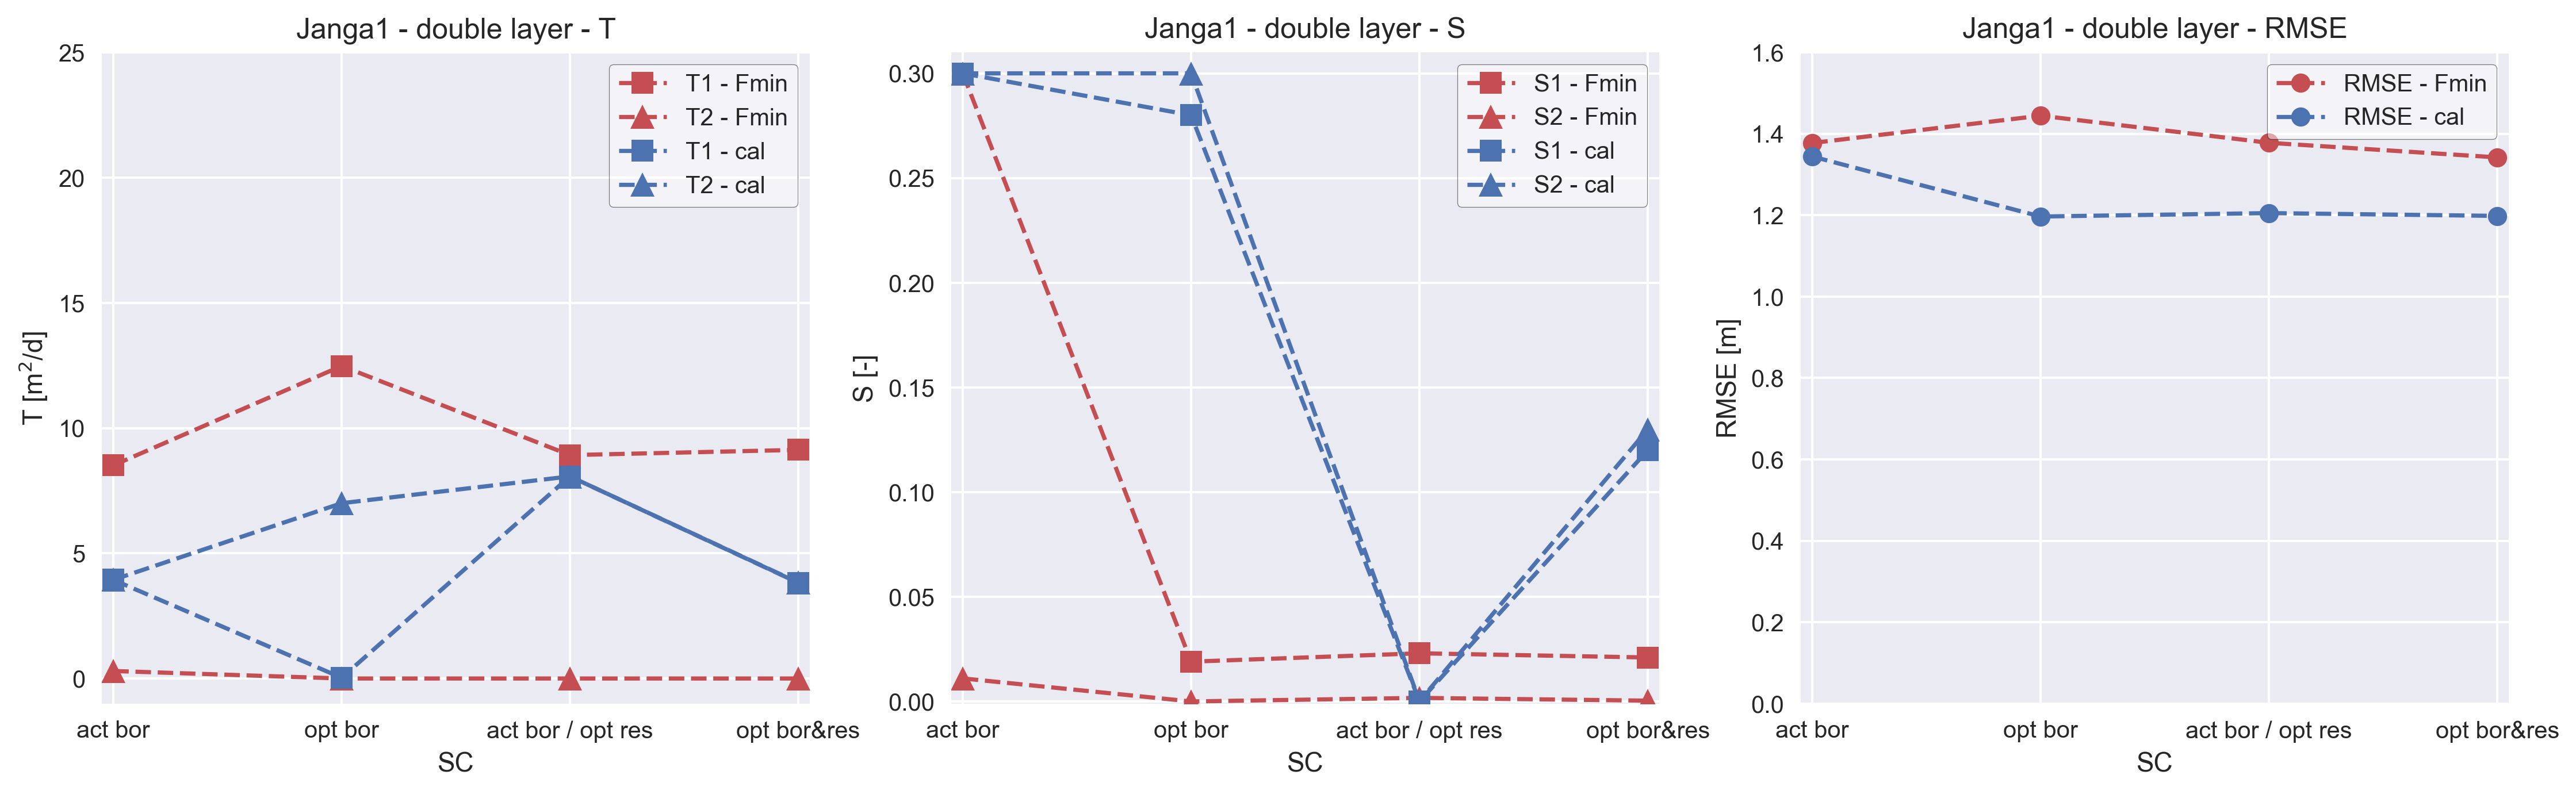
\includegraphics[width=\linewidth]{J1_para_results_2lay}
		\captionsetup{justification=centering}		
		\caption{\label{fig:J1_para_results_2lay}}
		\end{subfigure}
	\begin{subfigure}[b]{\linewidth}
		\centering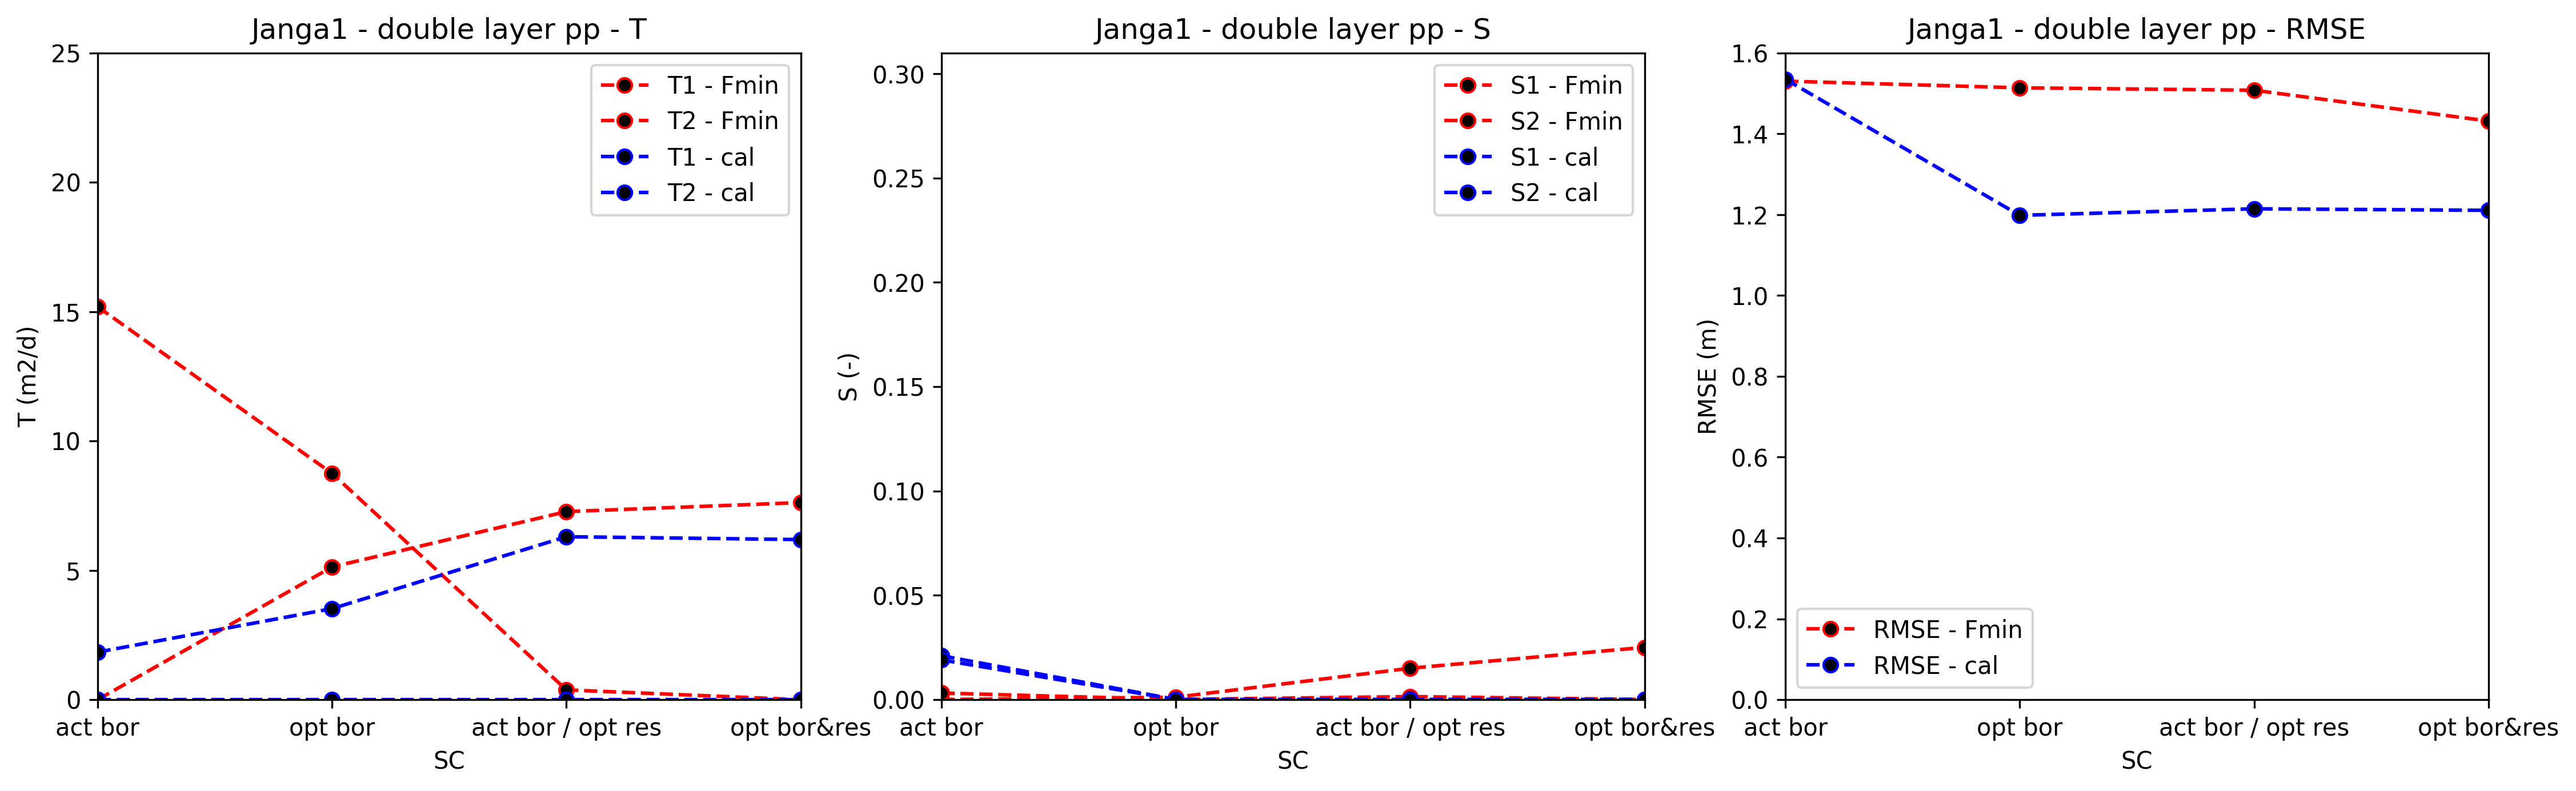
\includegraphics[width=\linewidth]{J1_para_results_3lay}
		\captionsetup{justification=centering}		
		\caption{\label{fig:J1_para_results_3lay}}
		\end{subfigure}		
	\captionsetup{justification=centering}	
	\caption{Janga first attempt - overview determined (Fmin and Cal) optimal parameter values of (\subref{fig:J1_para_results_1lay}) a single layer system, (\subref{fig:J1_para_results_2lay}) a double layer system, and (\subref{fig:J1_para_results_3lay}) a system with two layers and partial penetration of the well} 
	\label{fig:J1_para_results}
\end{figure} 

\clearpage\subsection{Location: Janga (2/2)}
\label{subsec:Janga2_overview}

\begin{figure}[h!]
	\centering
	\begin{subfigure}[b]{0.64\linewidth}
		\centering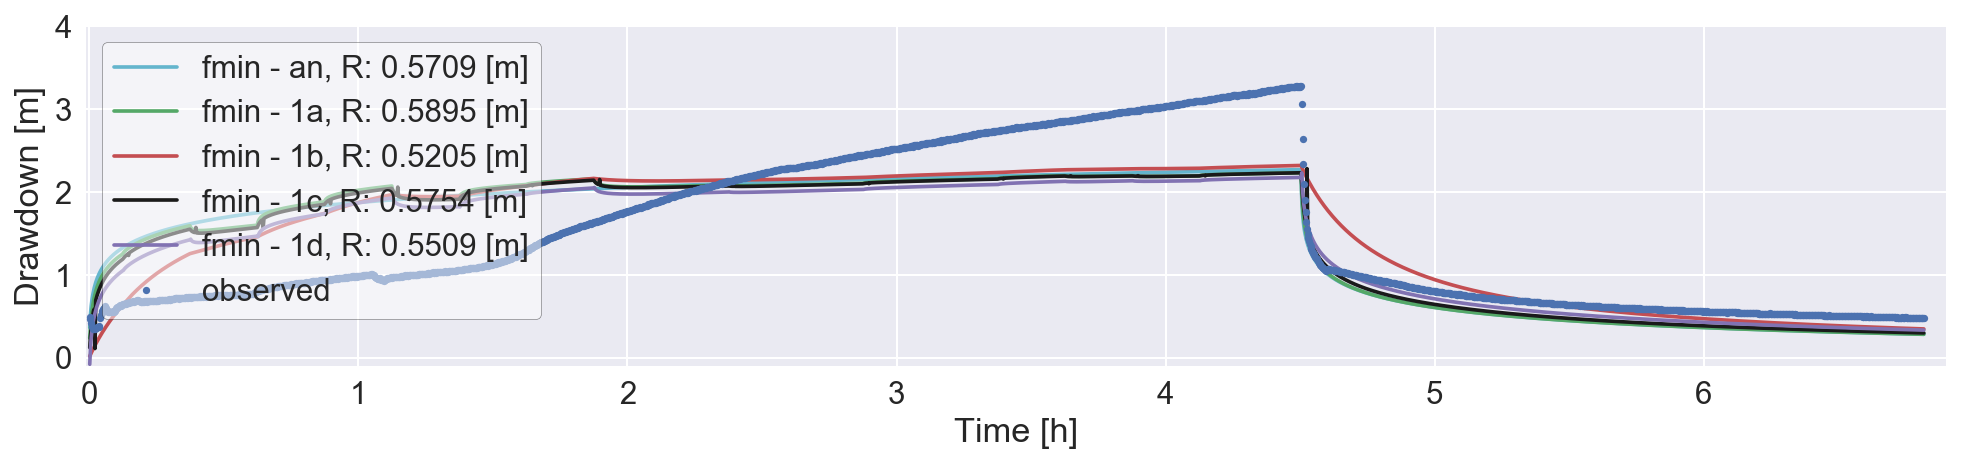
\includegraphics[width=\linewidth]{Janga2_1lay_fmin}
		\captionsetup{justification=centering}		
		\caption{\label{fig:Janga2_1lay_fmin}}
		\end{subfigure}\vfill
	\begin{subfigure}[b]{0.64\linewidth}
		\centering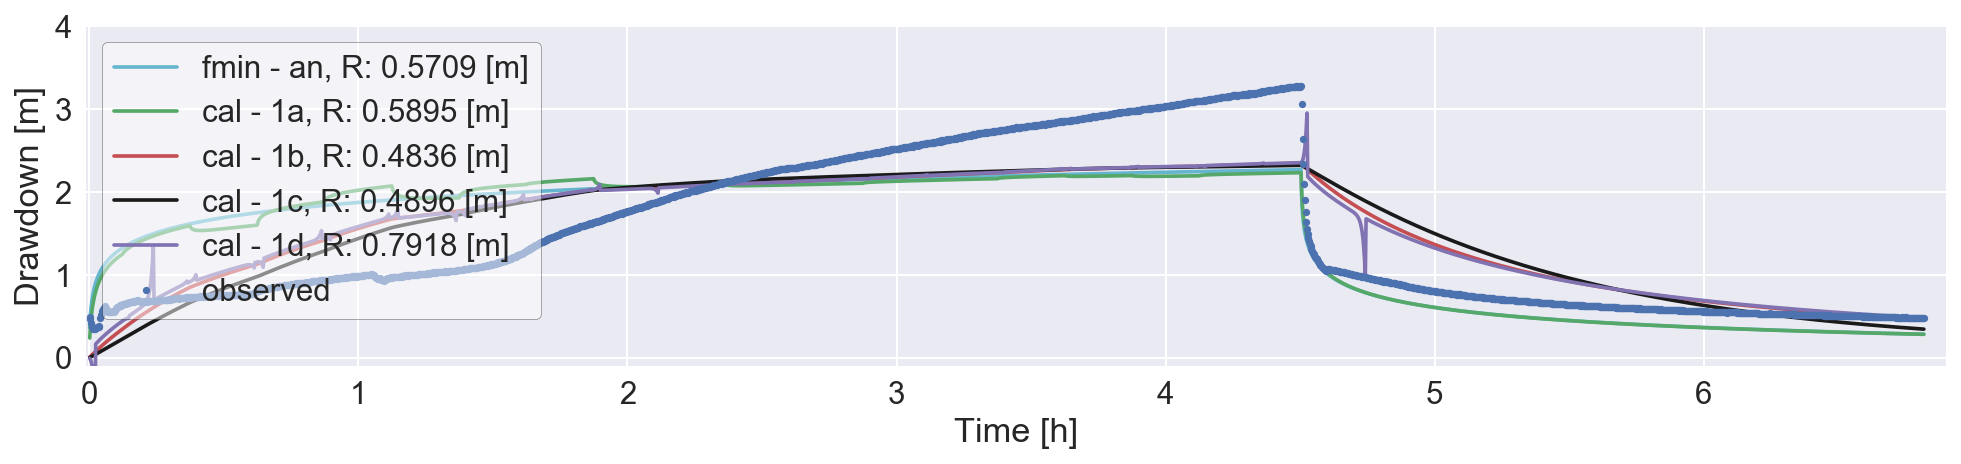
\includegraphics[width=\linewidth]{Janga2_1lay_cal}
		\captionsetup{justification=centering}		
		\caption{\label{fig:Janga2_1lay_cal}}
		\end{subfigure}
	\captionsetup{justification=centering}	
	\caption{Janga second attempt single layer fieldwork data analysis by the optimization (\subref{fig:Janga2_1lay_fmin}) fmin-RMSE method and (\subref{fig:Janga2_1lay_cal}) TTim calibration method} 
	\label{fig:Janga2_1lay_analysis}
\end{figure} 

\begin{figure}[h!]
	\centering
	\begin{subfigure}[b]{0.64\linewidth}
		\centering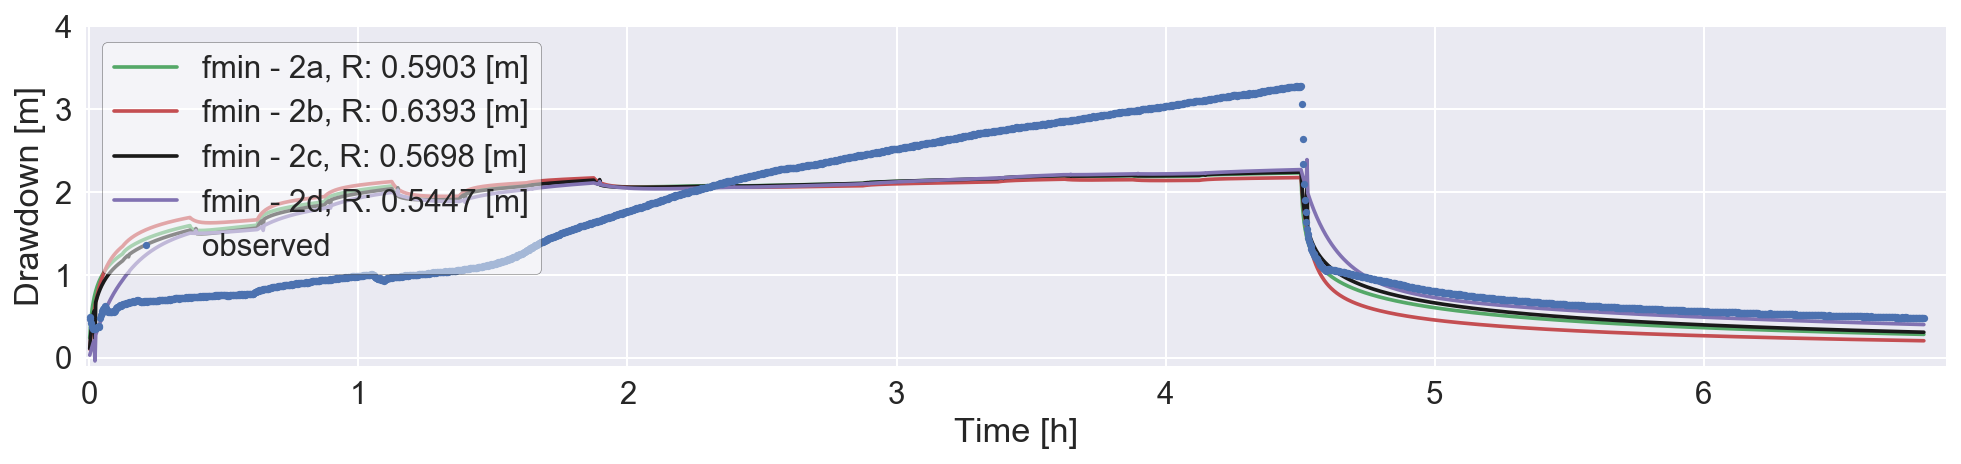
\includegraphics[width=\linewidth]{Janga2_2lay_fmin}
		\captionsetup{justification=centering}		
		\caption{\label{fig:Janga2_2lay_fmin}}
		\end{subfigure}\vfill
	\begin{subfigure}[b]{0.64\linewidth}
		\centering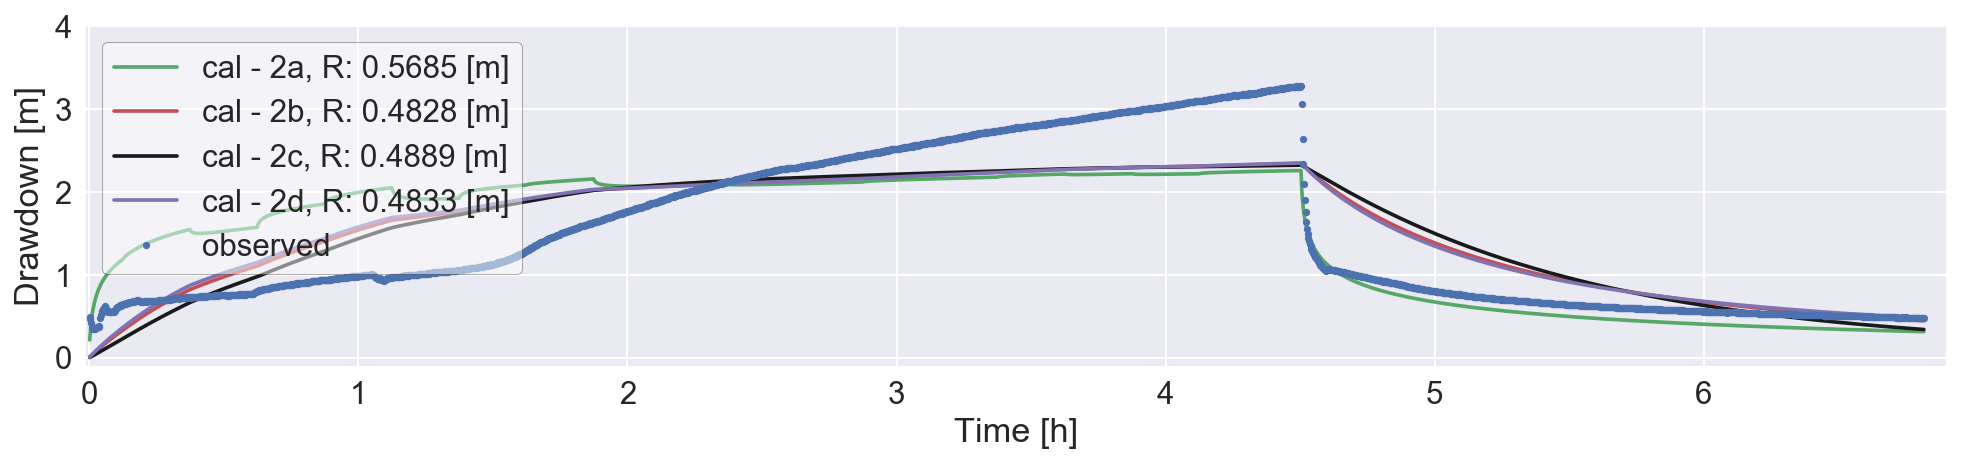
\includegraphics[width=\linewidth]{Janga2_2lay_cal}
		\captionsetup{justification=centering}		
		\caption{\label{fig:Janga2_2lay_cal}}
		\end{subfigure}
	\captionsetup{justification=centering}	
	\caption{Janga second attempt double layer fieldwork data analysis by the optimization (\subref{fig:Janga2_2lay_fmin}) fmin-RMSE method and (\subref{fig:Janga2_2lay_cal}) TTim calibration method} 
	\label{fig:Janga2_2lay_analysis}
\end{figure} 

\begin{figure}[h!]
	\centering
	\begin{subfigure}[b]{0.64\linewidth}
		\centering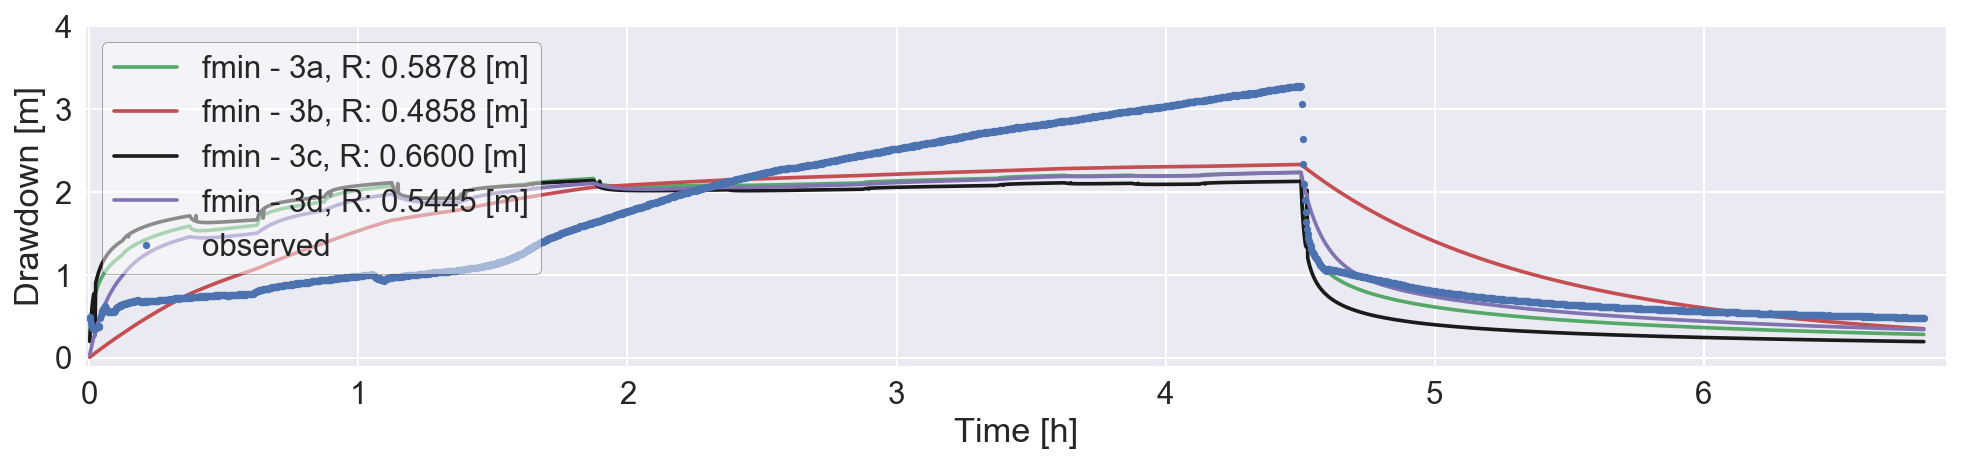
\includegraphics[width=\linewidth]{Janga2_3lay_fmin}
		\captionsetup{justification=centering}		
		\caption{\label{fig:Janga2_3lay_fmin}}
		\end{subfigure}\vfill
	\begin{subfigure}[b]{0.64\linewidth}
		\centering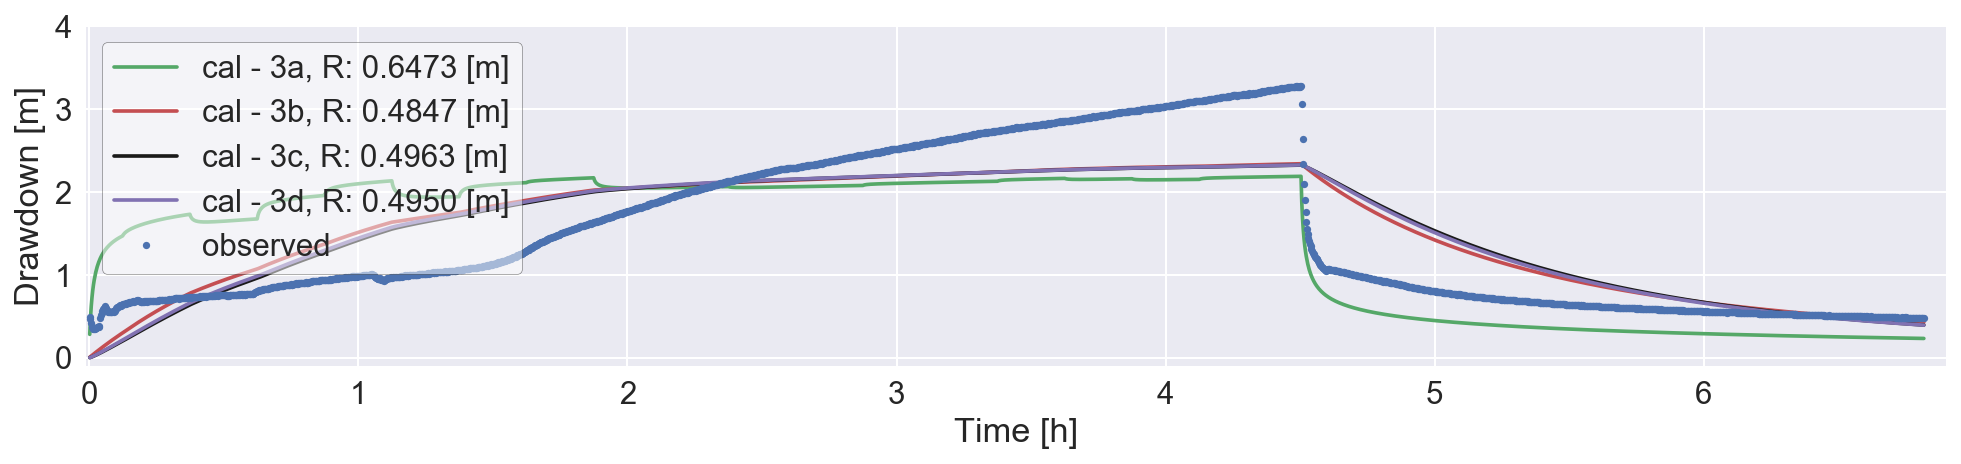
\includegraphics[width=\linewidth]{Janga2_3lay_cal}
		\captionsetup{justification=centering}		
		\caption{\label{fig:Janga2_3lay_cal}}
		\end{subfigure}
	\captionsetup{justification=centering}	
	\caption{Janga second attempt partially penetrating double layer fieldwork data analysis by the optimization (\subref{fig:Janga2_3lay_fmin}) fmin-RMSE method and (\subref{fig:Janga2_3lay_cal}) TTim calibration method} 
	\label{fig:Janga2_3lay_analysis}
\end{figure} 

\clearpage

\begin{figure}[h!]
	\centering
	\begin{subfigure}[b]{\linewidth}
		\centering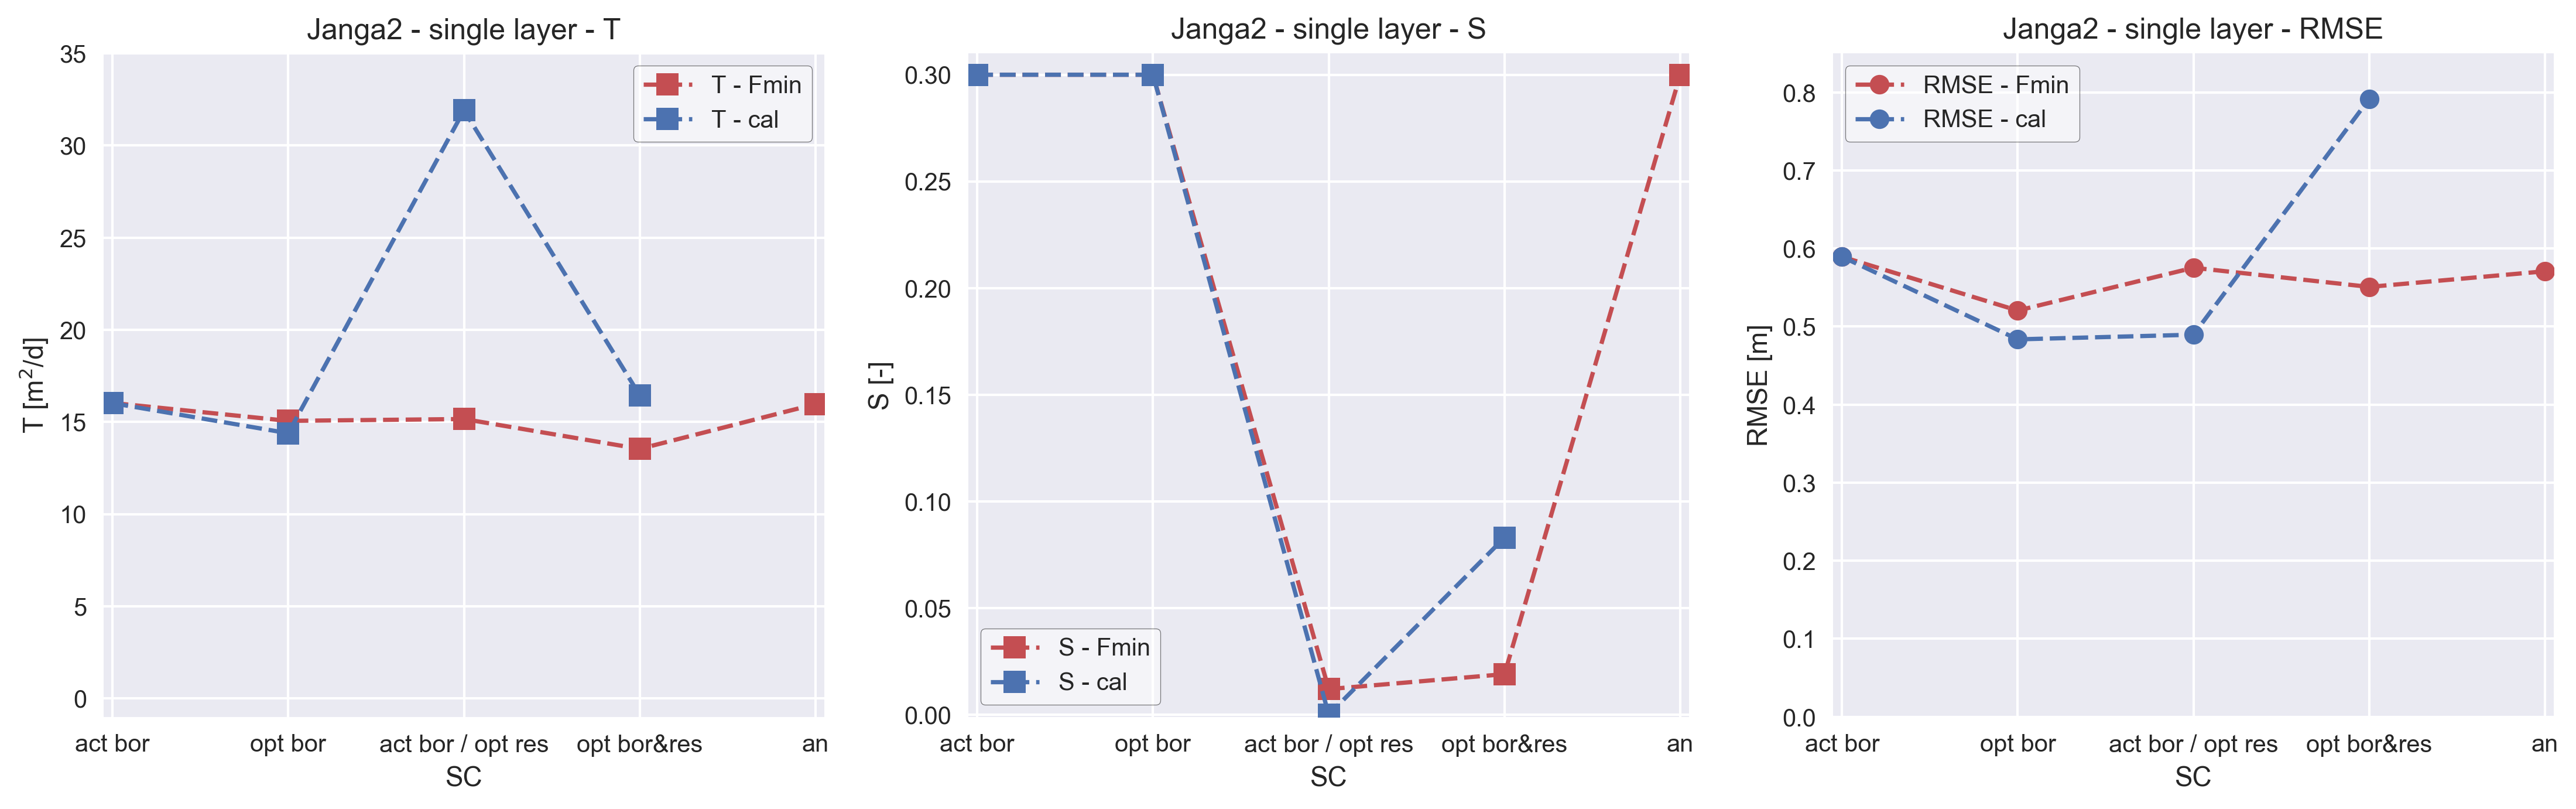
\includegraphics[width=\linewidth]{J2_para_results_1lay}
		\captionsetup{justification=centering}		
		\caption{\label{fig:J2_para_results_1lay}}
		\end{subfigure}\vfill
	\begin{subfigure}[b]{\linewidth}
		\centering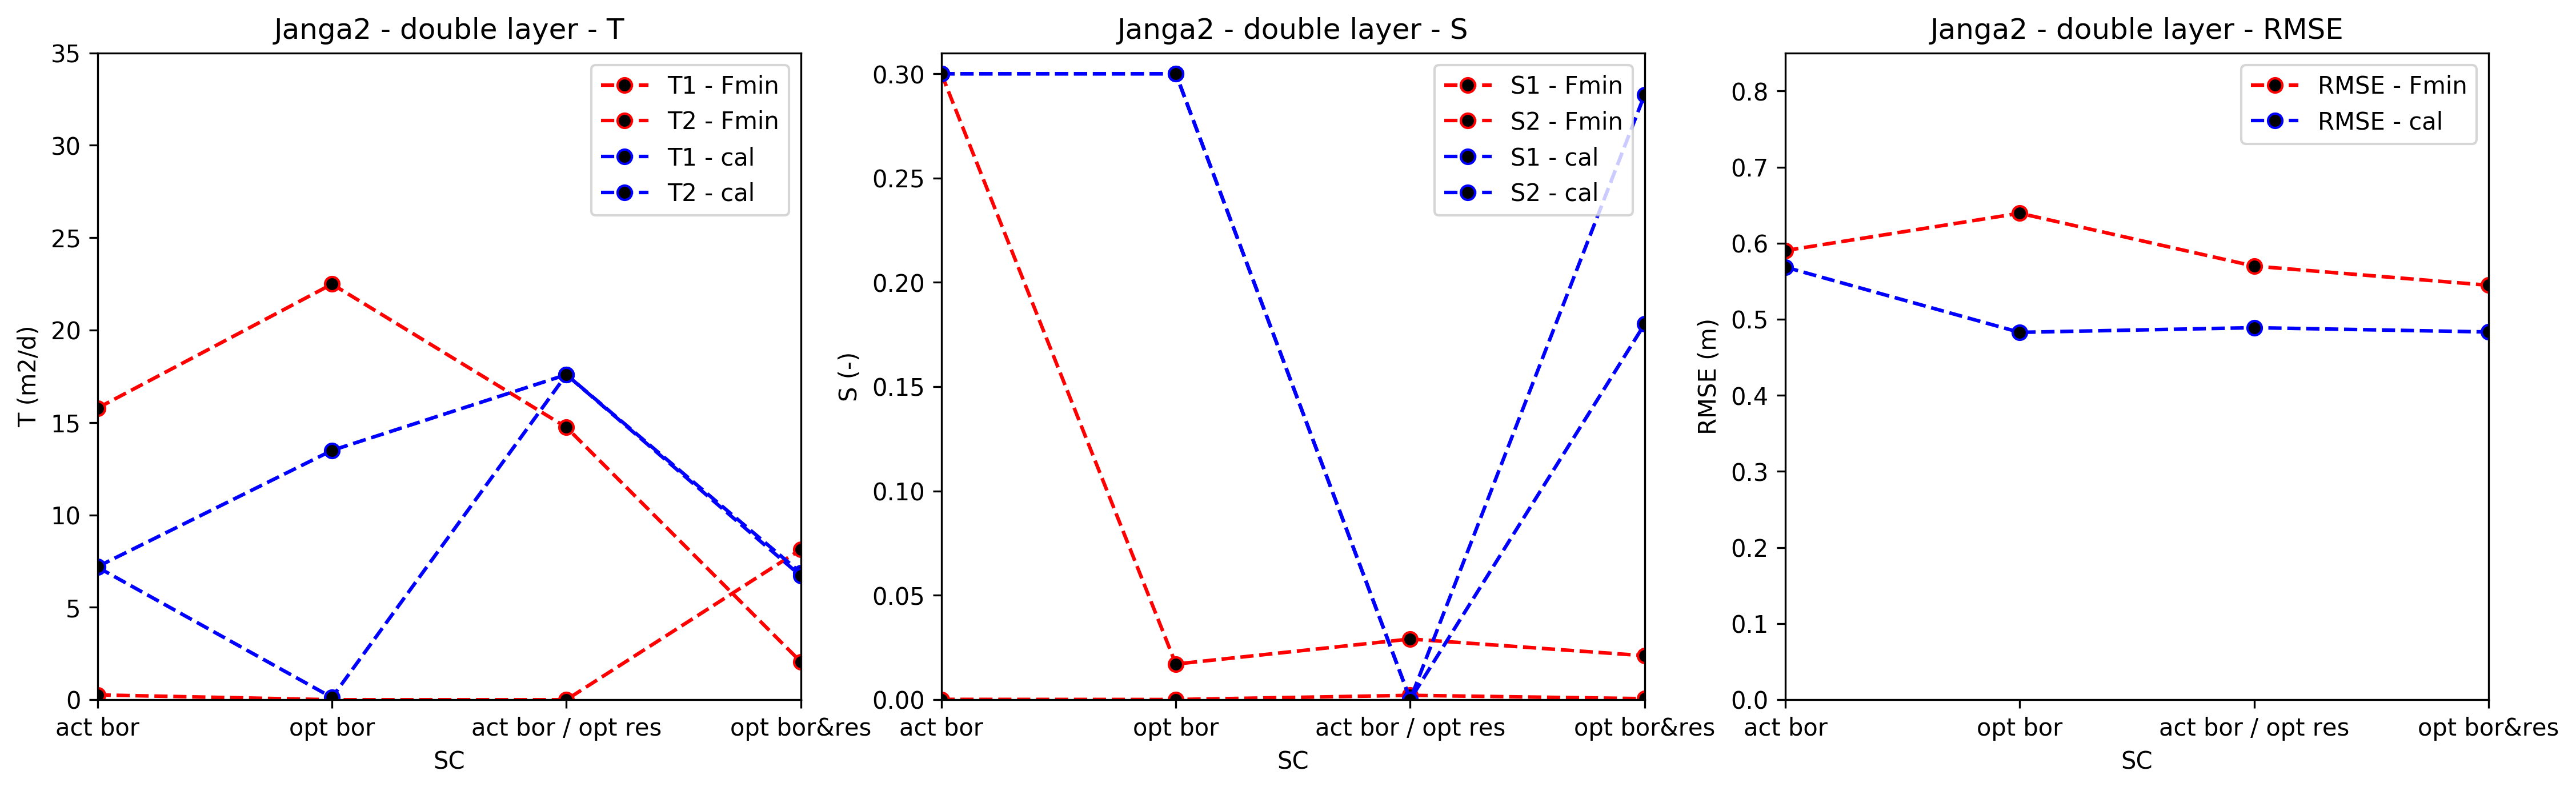
\includegraphics[width=\linewidth]{J2_para_results_2lay}
		\captionsetup{justification=centering}		
		\caption{\label{fig:J2_para_results_2lay}}
		\end{subfigure}
	\begin{subfigure}[b]{\linewidth}
		\centering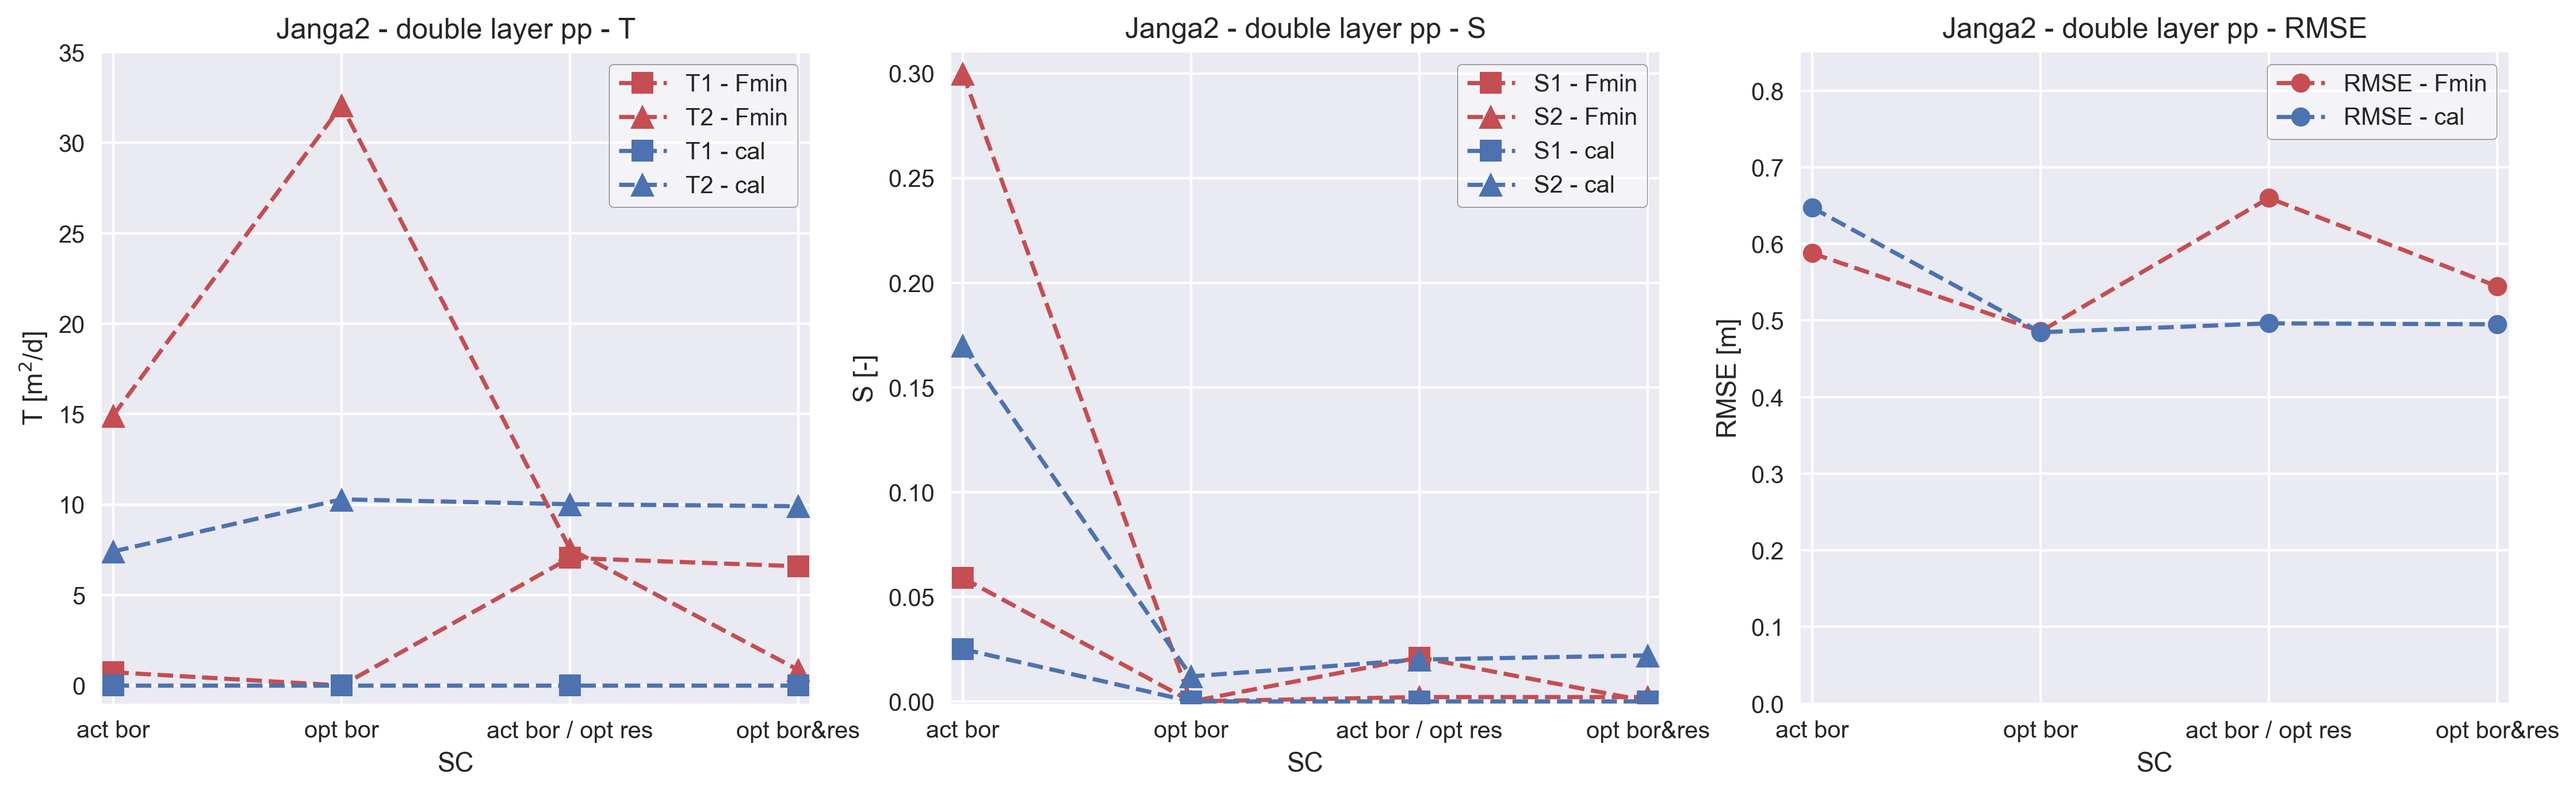
\includegraphics[width=\linewidth]{J2_para_results_3lay}
		\captionsetup{justification=centering}		
		\caption{\label{fig:J2_para_results_3lay}}
		\end{subfigure}		
	\captionsetup{justification=centering}	
	\caption{Janga second attempt - overview determined (Fmin and Cal) optimal parameter values of (\subref{fig:J2_para_results_1lay}) a single layer system, (\subref{fig:J2_para_results_2lay}) a double layer system, and (\subref{fig:J2_para_results_3lay}) a system with two layers and partial penetration of the well} 
	\label{fig:J2_para_results}
\end{figure} 


\clearpage\subsection{Location: Ziong}
\label{subsec:Ziong_overview}

\begin{figure}[h!]
	\centering
	\begin{subfigure}[b]{0.65\linewidth}
		\centering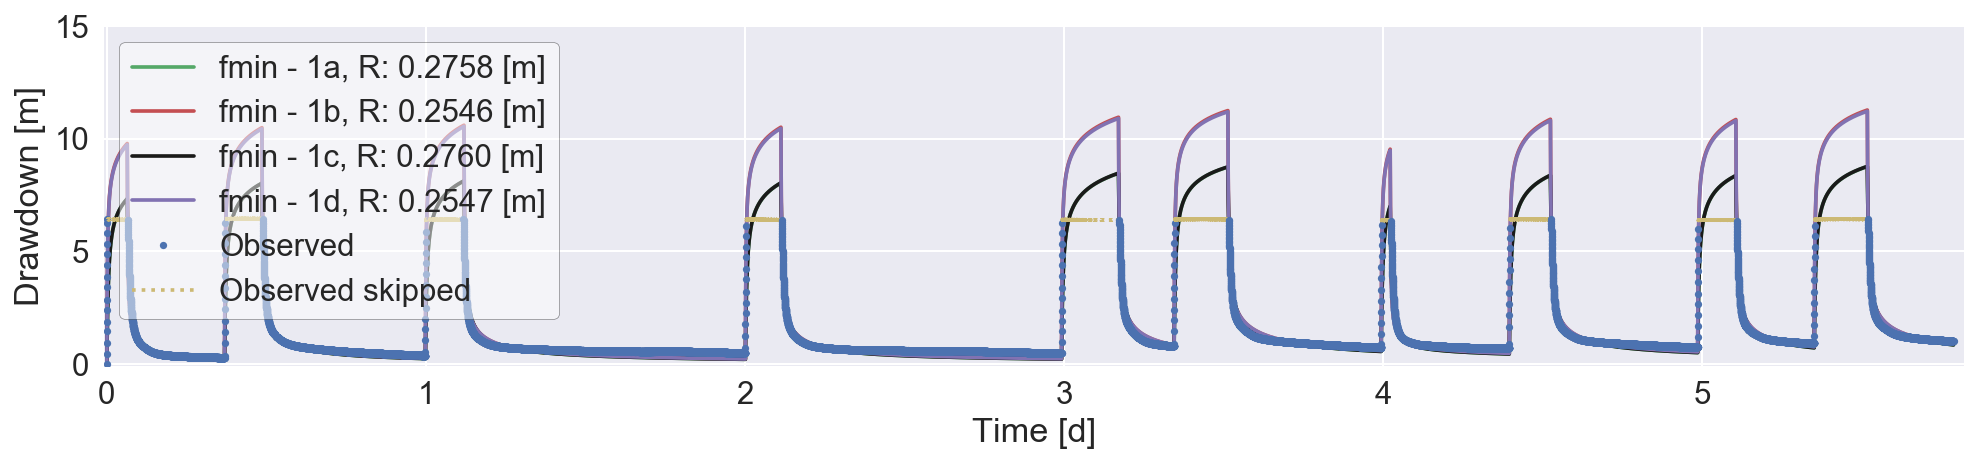
\includegraphics[width=\linewidth]{Ziong_1lay_fmin}
		\captionsetup{justification=centering}		
		\caption{\label{fig:Ziong_1lay_fmin}}
		\end{subfigure}\vfill
	\begin{subfigure}[b]{0.65\linewidth}
		\centering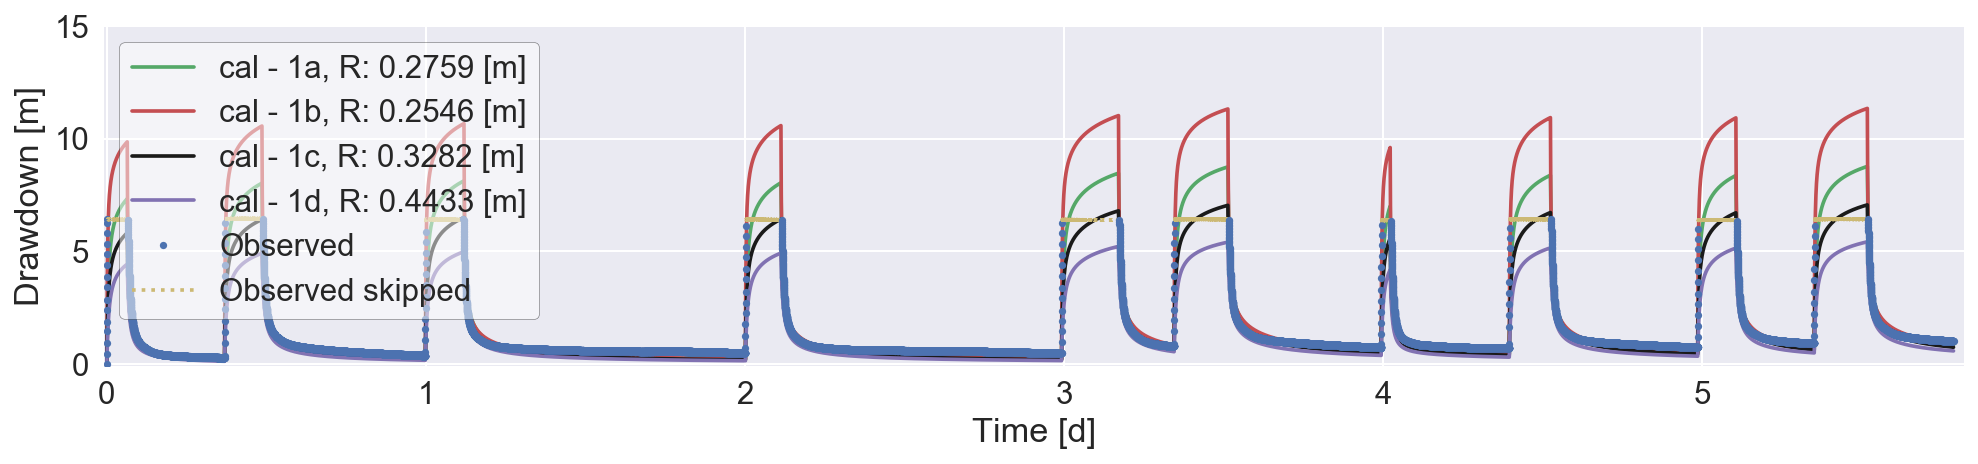
\includegraphics[width=\linewidth]{Ziong_1lay_cal}
		\captionsetup{justification=centering}		
		\caption{\label{fig:Ziong_1lay_cal}}
		\end{subfigure}
	\captionsetup{justification=centering}	
	\caption{Ziong single layer fieldwork data analysis by the optimization (\subref{fig:Ziong_1lay_fmin}) fmin-RMSE method and (\subref{fig:Ziong_1lay_cal}) TTim calibration method} 
	\label{fig:Ziong_1lay_analysis}
\end{figure} 

\begin{figure}[h!]
	\centering
	\begin{subfigure}[b]{0.65\linewidth}
		\centering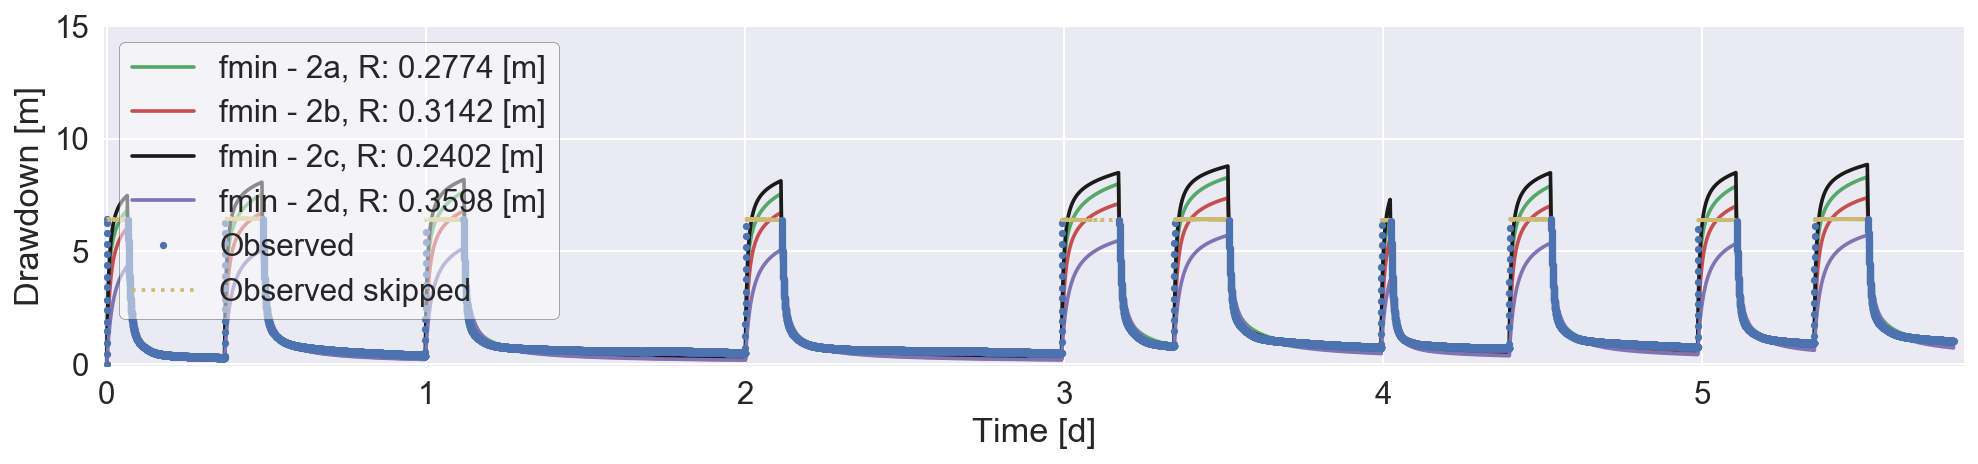
\includegraphics[width=\linewidth]{Ziong_2lay_fmin}
		\captionsetup{justification=centering}		
		\caption{\label{fig:Ziong_2lay_fmin}}
		\end{subfigure}\vfill
	\begin{subfigure}[b]{0.65\linewidth}
		\centering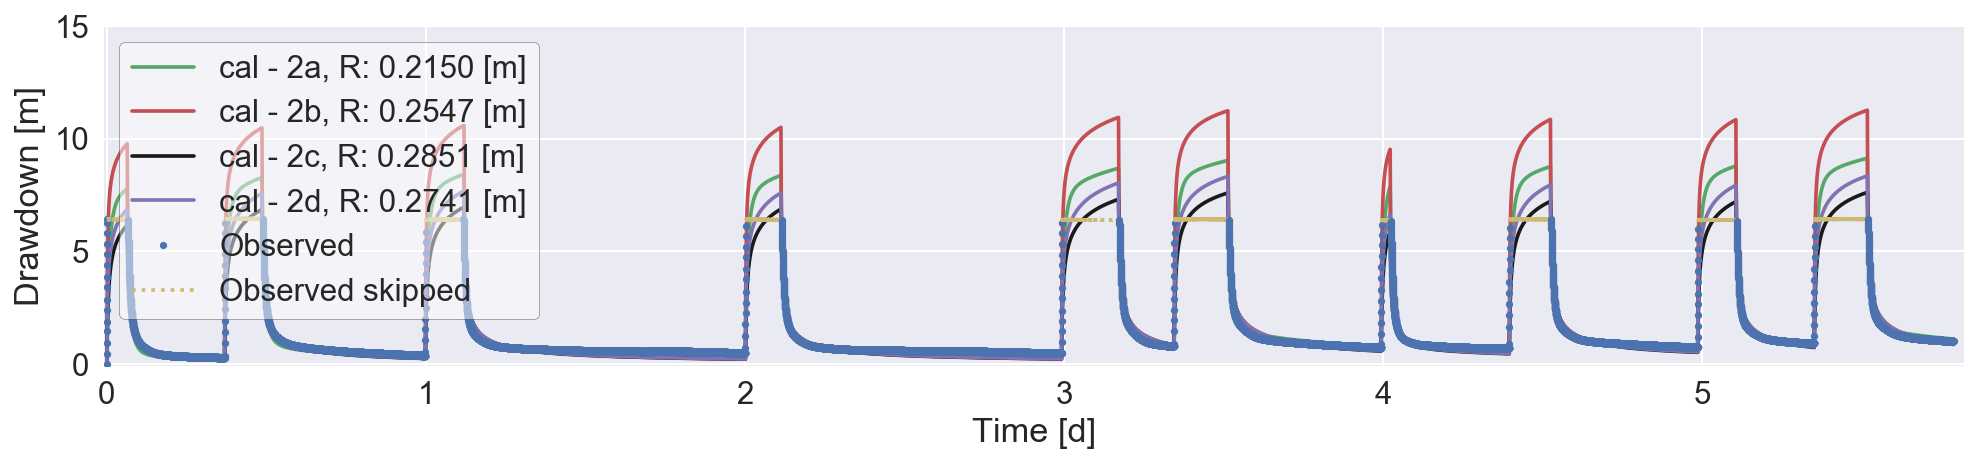
\includegraphics[width=\linewidth]{Ziong_2lay_cal}
		\captionsetup{justification=centering}		
		\caption{\label{fig:Ziong_2lay_cal}}
		\end{subfigure}
	\captionsetup{justification=centering}	
	\caption{Ziong double layer fieldwork data analysis by the optimization (\subref{fig:Ziong_2lay_fmin}) fmin-RMSE method and (\subref{fig:Ziong_2lay_cal}) TTim calibration method} 
	\label{fig:Ziong_2lay_analysis}
\end{figure} 

\begin{figure}[h!]
	\centering
	\begin{subfigure}[b]{0.65\linewidth}
		\centering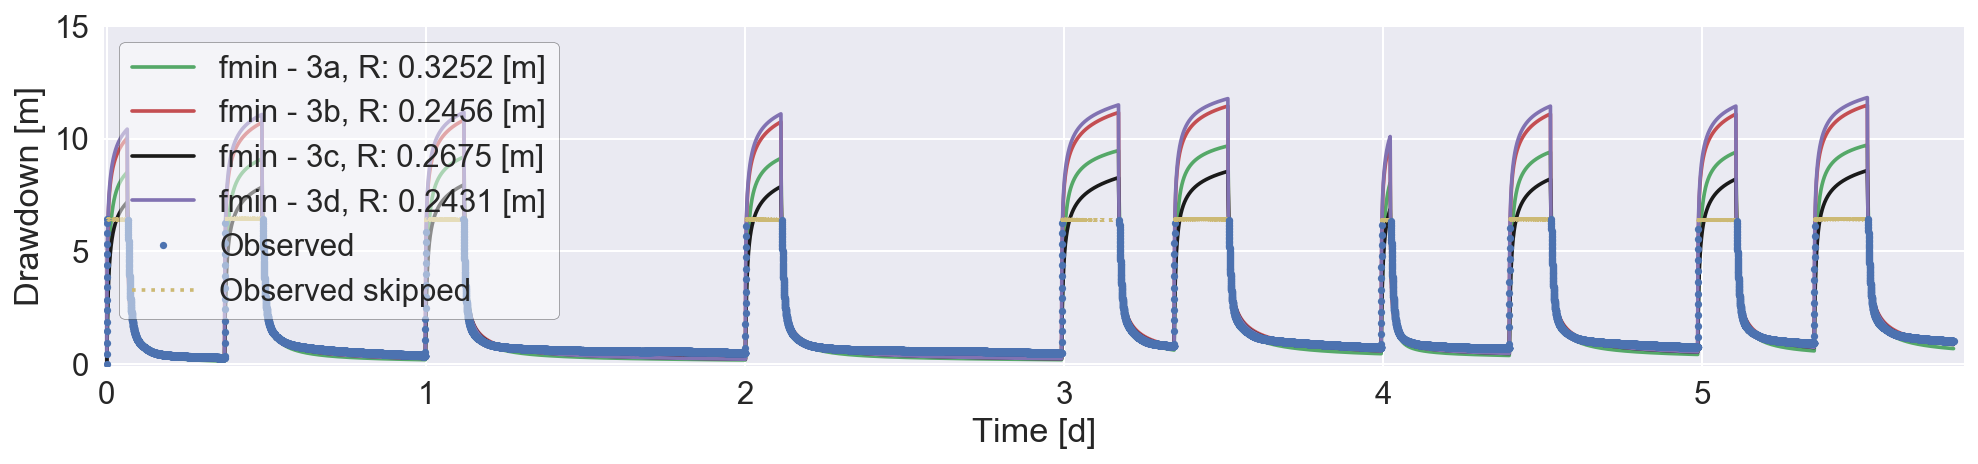
\includegraphics[width=\linewidth]{Ziong_3lay_fmin}
		\captionsetup{justification=centering}		
		\caption{\label{fig:Ziong_3lay_fmin}}
		\end{subfigure}\vfill
	\begin{subfigure}[b]{0.65\linewidth}
		\centering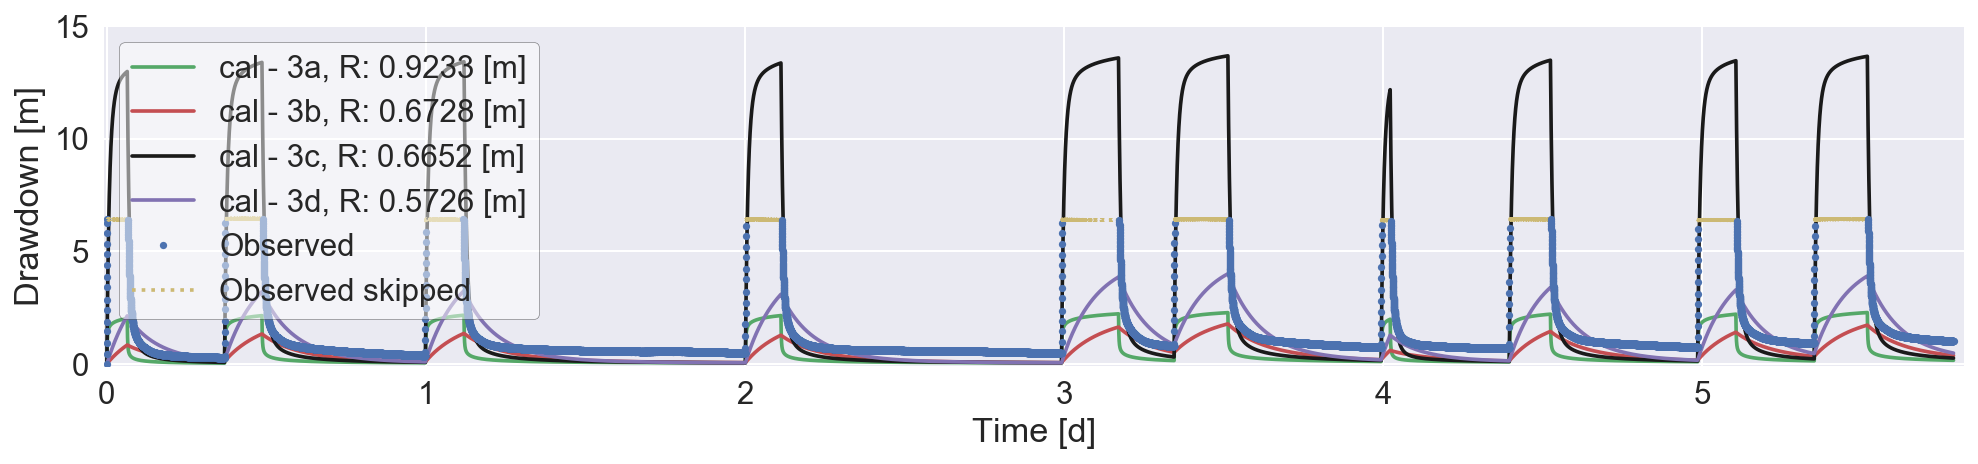
\includegraphics[width=\linewidth]{Ziong_3lay_cal}
		\captionsetup{justification=centering}		
		\caption{\label{fig:Ziong_3lay_cal}}
		\end{subfigure}
	\captionsetup{justification=centering}	
	\caption{Ziong partially penetrating double layer fieldwork data analysis by the optimization (\subref{fig:Ziong_3lay_fmin}) fmin-RMSE method and (\subref{fig:Ziong_3lay_cal}) TTim calibration method} 
	\label{fig:Ziong_3lay_analysis}
\end{figure} 

\clearpage

\begin{figure}[h!]
	\centering
	\begin{subfigure}[b]{\linewidth}
		\centering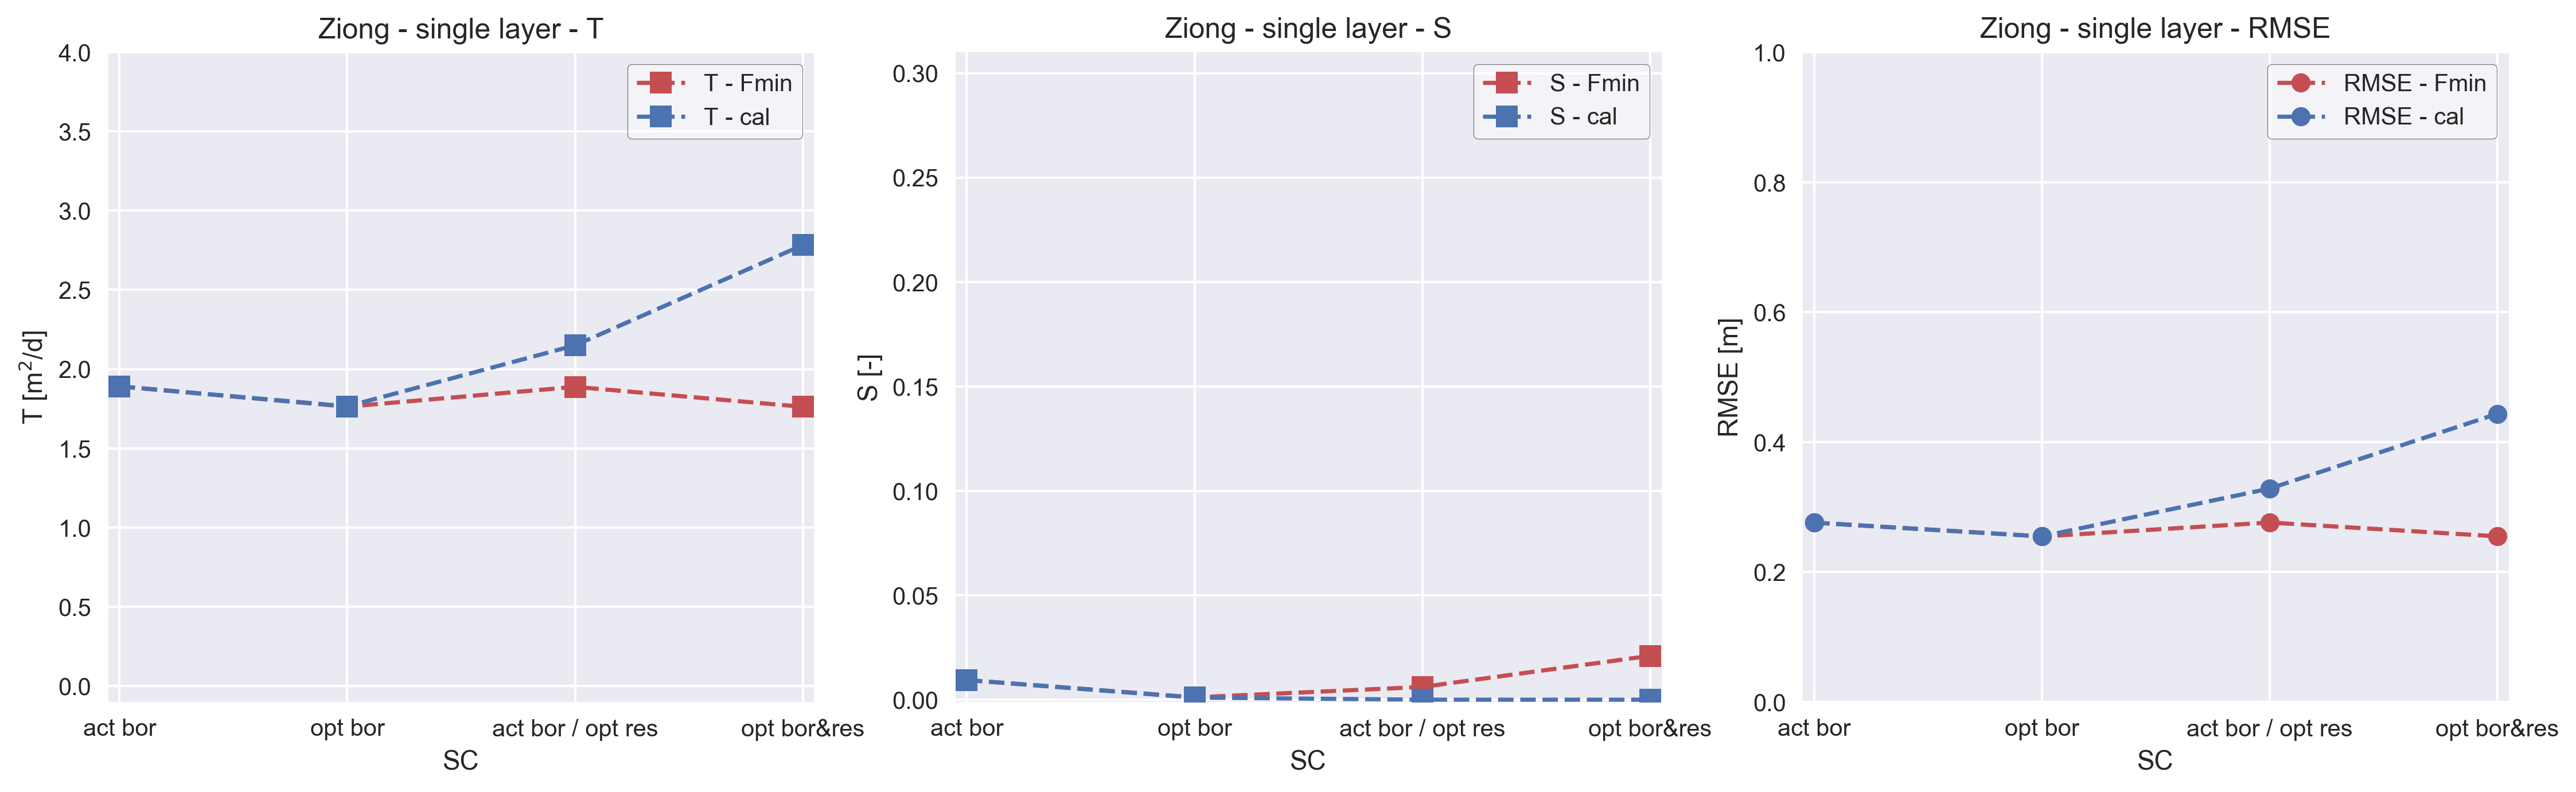
\includegraphics[width=\linewidth]{Ziong_para_results_1lay}
		\captionsetup{justification=centering}		
		\caption{\label{fig:Ziong_para_results_1lay}}
		\end{subfigure}\vfill
	\begin{subfigure}[b]{\linewidth}
		\centering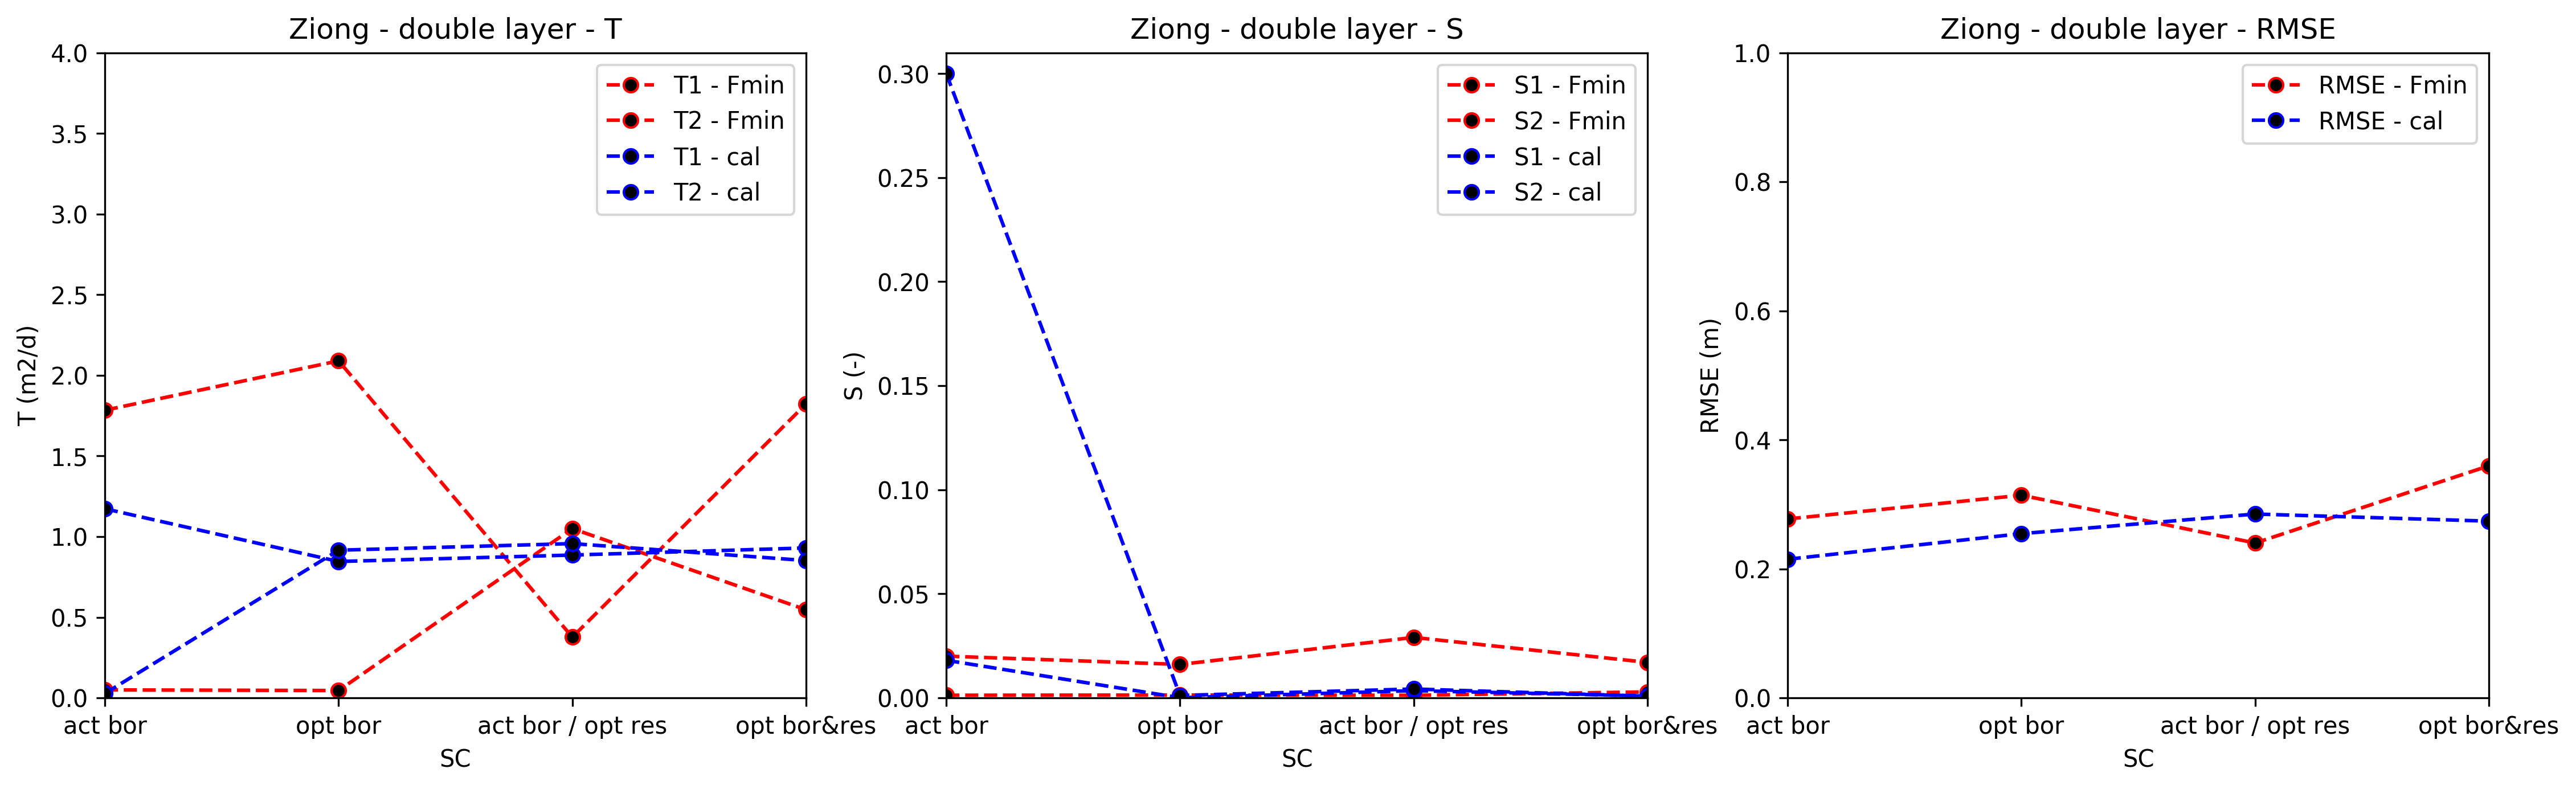
\includegraphics[width=\linewidth]{Ziong_para_results_2lay}
		\captionsetup{justification=centering}		
		\caption{\label{fig:Ziong_para_results_2lay}}
		\end{subfigure}
	\begin{subfigure}[b]{\linewidth}
		\centering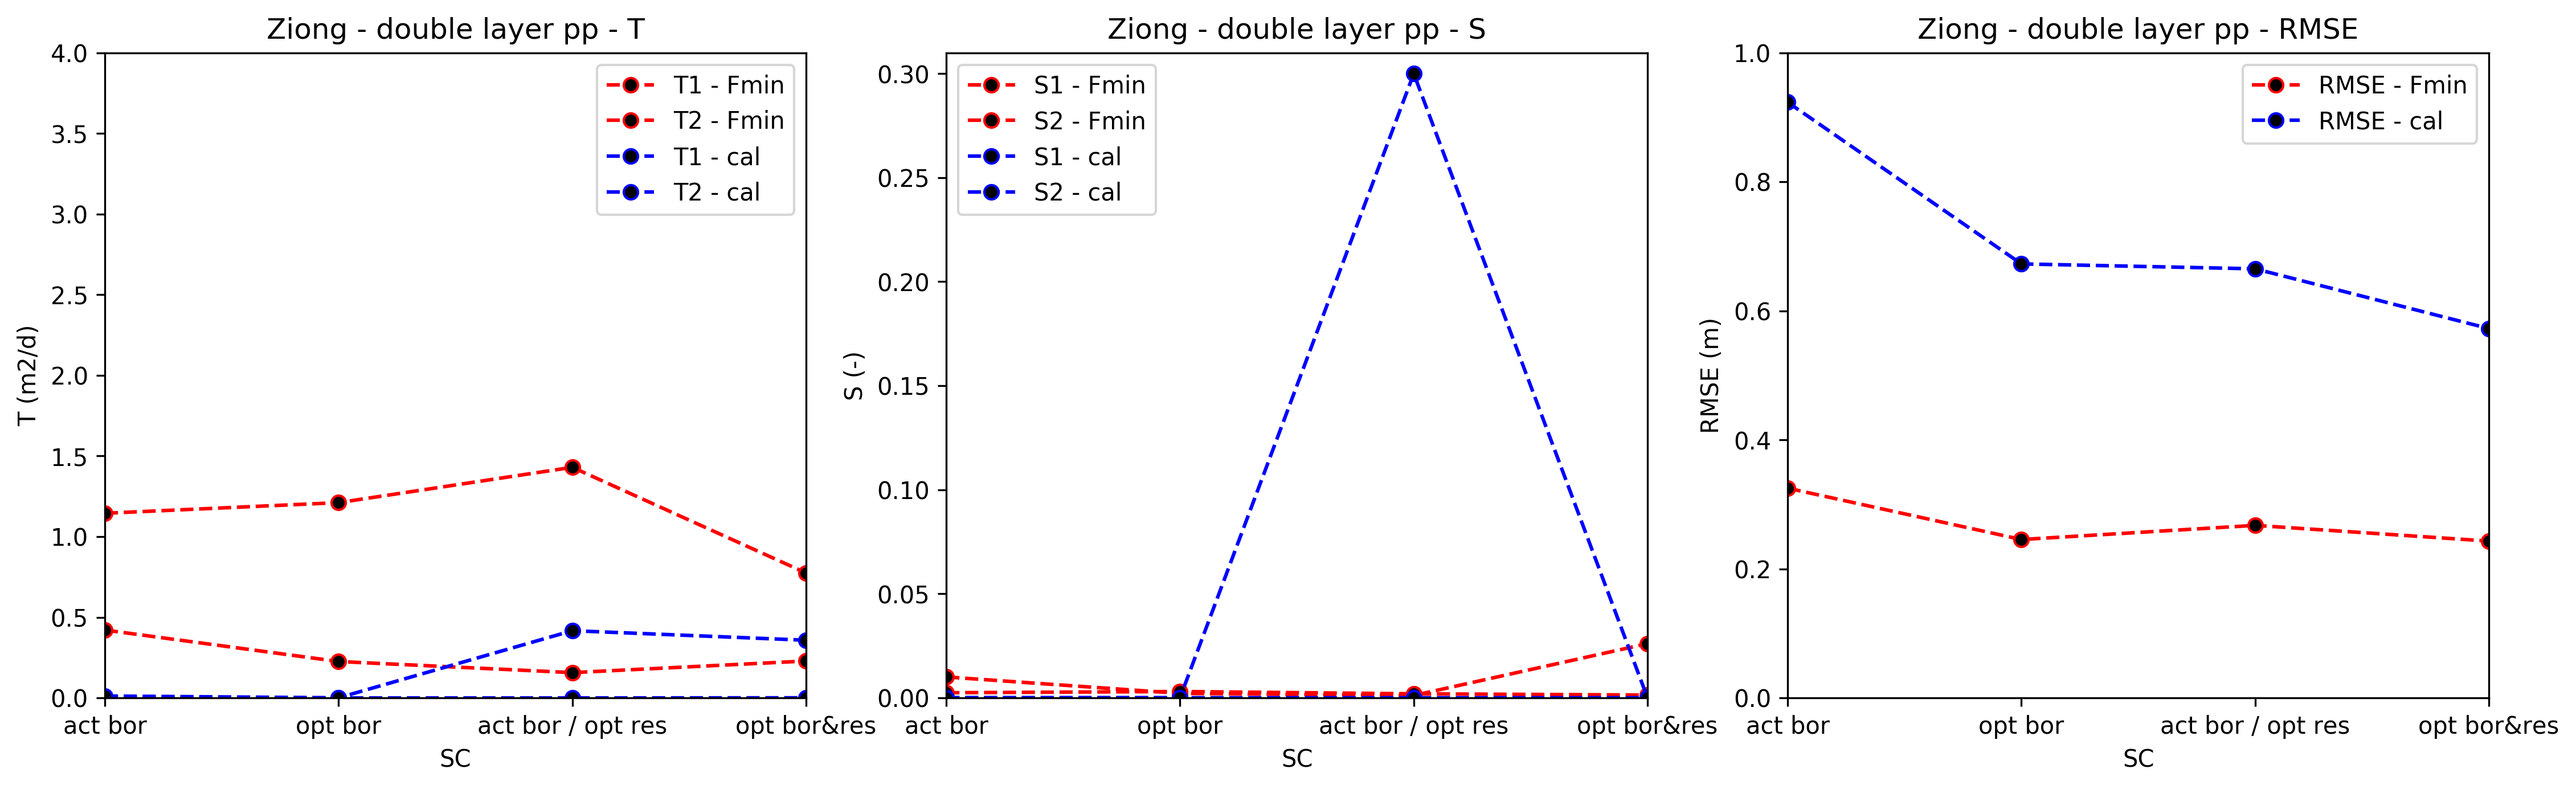
\includegraphics[width=\linewidth]{Ziong_para_results_3lay}
		\captionsetup{justification=centering}		
		\caption{\label{fig:Ziong_para_results_3lay}}
		\end{subfigure}		
	\captionsetup{justification=centering}	
	\caption{Ziong - overview determined (Fmin and Cal) optimal parameter values of (\subref{fig:Ziong_para_results_1lay}) a single layer system, (\subref{fig:Ziong_para_results_2lay}) a double layer system, and (\subref{fig:Ziong_para_results_3lay}) a system with two layers and partial penetration of the well} 
	\label{fig:Ziong_para_results}
\end{figure} 
